\documentclass[10pt]{article}

\usepackage[T1]{fontenc}
\usepackage[utf8]{inputenc}
\usepackage{lmodern}
\usepackage{amsmath}
\usepackage{amssymb}
\usepackage{pifont}
\usepackage{bm}
\usepackage{graphicx}
\usepackage[space]{grffile}
\usepackage{multicol}
\usepackage{array}
\usepackage{tabu}
\usepackage{ragged2e}
\usepackage{setspace}
\usepackage{xr} % package for linking external document references
\usepackage[font=small,labelfont=bf,labelsep=period]{caption}
%\usepackage{subcaption}
%\usepackage[CaptionAfterwards]{fltpage}
\usepackage{lineno}
\linenumbers
\usepackage{tikz}
\usepackage[margin=1.0in]{geometry}

\usepackage[backend=biber,style=authoryear,sorting=nyt,url=false,isbn=false,doi=false,firstinits=true]{biblatex}

\DeclareNameAlias{default}{last-first}

\DefineBibliographyStrings{english}{%
	andothers = {\addcomma\addspace\textsc{et\addabbrvspace al}\adddot},
	and = {\textsc{and}}
}
\renewcommand*{\labelnamepunct}{\space\space}

\renewbibmacro{in:}
{%
	\ifentrytype{article}{%
	}{%
		\printtext{\bibstring{in}\intitlepunct}%
	}%
}
\renewbibmacro*{volume+number}{%
	\printfield{volume}%
	\setunit*{\addcomma\space}%
	\printfield{number}%
	\setunit{\addcomma\space}}

\DeclareFieldFormat{pages}{#1}

\renewbibmacro*{publisher+location+date}{%
	\printlist{publisher}%
	\setunit*{\addcomma\space}%
	\setunit*{\addcomma\space}%
	\usebibmacro{date}%
	\newunit}

\renewcommand{\newunitpunct}{\addcomma\space}
\DeclareFieldFormat[article,inbook,incollection,inproceedings,patent,thesis,unpublished]{title}{#1} 
\DeclareFieldFormat{year}{#1} 

\renewcommand{\baselinestretch}{2.0}
\addbibresource{refs/ident_refs.bib}
\captionsetup{font={stretch=2.0}}
\externaldocument{sifigures} % reference to existing external document

\begin{document}
	\begin{center}
		\begin{Large}
			Practical Identification and Experimental Design for Parameter Estimation in Kinetic Models of Metabolism
		\end{Large}\\
		Shyam Srinivasan\textsuperscript{a}, William R. Cluett\textsuperscript{a} and Radhakrishnan Mahadevan\textsuperscript{*,a,b}\\
	\end{center}
	a - Department of Chemical Engineering and Applied Chemistry, University of Toronto, Toronto, ON, Canada.\\
	b - Institute for Biomaterials and Biomedical Engineering, University of Toronto, Toronto, ON, Canada.\\
	{*} Corresponding author
	\section*{Abstract}
	\section{Introduction:}
	The use of metabolic engineering spans a wide variety of applications. Some notable examples include the design of microorganisms for the biosynthesis of commodity and specialty chemicals \parencite{Andreozzi2016}, engineering mammalian cells as therapeutic targets for cures to some ailments affecting humans \parencite{DiFilippo2016,Apaolaza2017}, and changing the constituents of the human gut microbial community to cure related diseases \parencite{Zerfab2018}. These applications require us to understand the numerous complex interactions, their roles in cell function, and sometimes even the mechanisms behind these interactions. Computational models offer a systematic way to integrate available experimental data, and to study and understand these interactions through mathematical representations of the biological systems in which these interactions occur \parencite{Bordbar2014a,Saa2017}. They are also used to predict changes in cell function based on changes in the type and nature of the modeled interactions \parencite{Andreozzi2016}, or aid in the identification of therapeutic targets for drug discovery and development \parencite{Bordbar2015,Chandrasekaran2017}
	
	Constraint-based models (CBMs) of metabolism are used to improve our understanding of metabolism by representing it as a stoichiometric network of reactions \parencite{Bordbar2014a}. The ability of CBMs to shine light on the nonintuitive interactions that govern cellular metabolism is leveraged to engineer and asses the impact of designs that alter the ability of a cell to grow, or produce a desired metabolite \parencite{Maia2016}. However, in CBMs, metabolism is assumed to operate under a pseudo steady state. Consequently, the metabolite concentrations within the metabolic network are assumed to be constant, and changes in metabolite concentrations are not modeled. Furthermore, since CBMs represent metabolism using only the stoichiometry of its constituent reactions, they do not account for the various non-catalytic regulatory interactions that are also responsible for metabolic function. These shortcomings prevent CBMs from being used to fully understand the steady state as well as the dynamic characteristics of metabolic networks. 
	
	In contrast, the effects of regulatory interactions and changes in metabolite concentrations on different characteristics of metabolism can be studied using kinetic models of metabolism \parencite{Saa2017}. These models account for changes in metabolite concentrations subject to thermodynamic and regulatory constraints that underly metabolic networks in addition to their stoichiometry \parencite{Link2014}. Kinetic models can not only help us better understand lesser known and understood characteristics of metabolism like bistability \parencite{Kotte2014}, and their role in human health, but can also improve predictions about the impact of engineering design perturbations on metabolism, and help propose alternative designs to achieve metabolite production goals \parencite{Khodayari2016}. 
	
	Kinetic models differ from CBMs in their use of mechanistic enzyme kinetics to model the fluxes within a metabolic network \parencite{Srinivasan2015,Saa2017}. The use of kinetic models requires information on the enzyme kinetic rate laws that will be used to model the fluxes, as well as numerical values for the parameters used in these rate laws. Analyzing the ability of a metabolic network to exhibit dynamic characteristics like multiple steady states and oscillations, irrespective of the structure of the network, is one example where kinetic rate laws and parameter values play a crucial role \parencite{Srinivasan2017}. 
	
	Despite their importance, the parameterization of kinetic models is still a problem for which solutions are a subject of debate within the modeling community. Typically, enzyme kinetic rate laws are parameterized based on in vitro observations of enzyme activity, as opposed to observations made under in vivo conditions \parencite{Heijnen2005,Smallbone2007}. However, some researchers have questioned their relevance for gleaning information on the dynamics of metabolism under in vivo conditions \parencite{Heijnen2005,Heijnen2013}. On the other hand, some reports have shown that despite the large uncertainties associated with parameters estimated based on in vivo experimental data \parencite{Link2014}, in vitro parameter estimates are a reasonable approximation of values that would be applicable under in vivo conditions \parencite{Davidi2016}. 
	
	Authors have sought to constrain and determine uncertainty in parameter estimates and associated model predictions by using Monte Carlo approaches for kinetic modeling of metabolism \parencite{Andreozzi2016a}. These approaches also allow for the integration of experimentally observed in vivo data. ORACLE \parencite{Wang2004} and Ensemble modeling \parencite{Tran2008} are two such examples. These, and other Monte Carlo kinetic modeling methods have been previously reviewed \parencite{Srinivasan2015}. Bayesian approaches to improve parameter estimation and quantify estimation uncertainty have also been proposed \parencite{Saa2016}. \textcite{Vanlier2013} provide a review of different Bayesian approaches to quantify parameter uncertainty.	 
	
	However, the importance of model parameter identifiability, i.e., a necessary condition to estimate unique kinetic parameter values from experimental data, is often overlooked \parencite{Rodriguez-Fernandez2006,Berthoumieux2013}. Unique parameter estimates from experimental data can only be obtained for structurally and practically identifiable parameters. 
	
	Briefly, it should be possible to obtain unique estimates for structurally identifiable parameters, just based on the model structure and parameterization, irrespective of the type and nature of experimental data available. If parameters cannot be uniquely estimated due to their nonlinear relationships with other parameters (redundant model parameterization), or due to the lack of a relationship between the measured concentrations/fluxes and the unmeasurable concentrations/fluxes (presence of unobservable system states) modeled by the parameters, then these parameters are said to be structurally non-identifiable.
	
	If the experimental data used for parameter estimation is informative so as to facilitate obtaining unique parameter estimates, or the quantification of uncertainties in the parameter estimates, then the parameters are said to be practically identifiable. However, if the ability to estimate unique parameter values is compromised due to the inability of the available data to capture the requisite information needed to estimate the parameters in the modeled system, or the uncertainty in parameter estimates is not quantifiable, the parameters are said to be practically non-identifiable. 
	
	Authors have proposed ways to assess parameter identifiability by proposing approximate kinetic models of metabolism that utilize empirical enzyme kinetic rate laws with parameters that have physical significance, and are identifiable \parencite{Heijnen2005,Smallbone2007}. Significant work has also been done towards the development of methods for structural identification of parameters in kinetic models of metabolism \parencite{Nikerel2009,Berthoumieux2013,Raue2014}. \textcite{Chis2011b} provide a comparison of the computational performance and implementation aspects of some of these methods. 
	
	Methods to improve practical identifiability through a priori experimental design have also been developed, with a focus on kinetic models of metabolism \parencite{Gadkar2005a,Rodriguez-Fernandez2006,Vanlier2014a,Raue2014}. Some of these methods are limited by their applicability to approximate kinetic models only \parencite{Nikerel2009,Berthoumieux2013}, while some others suffer from computational limitations when applied to kinetic models of large metabolic networks \parencite{Gadkar2005a,Raue2014}. 	
	Assessing the identifiability (structural or practical) of parameters using any of the aforementioned or other methods is done under the assumption that only dynamic time course concentration data is available and can be used for parameter estimation. The ability to use steady state experimental data to assess parameter identifiability is rarely addressed, and very few methodology have been proposed to fill this gap \textcolor{red}{(paper that proposes both steady state and dynamic data use for a priori experimental design resulting in reduced model sizes)} 	
	
	In this paper, we show that the identifiability of most parameters in a metabolic network can be done for each reaction individually using steady state fluxomics, metabolomics and proteomics data, and propose a methodology to do so. We also demonstrate how this method can facilitate the design of experiments for generating the necessary steady state data to estimate unique parameter values for all reaction fluxes in a metabolic network. In doing so, we are able to propose the number and types of perturbations that will provide the most useful data for parameter estimation. We also comment on the identifiability of different enzyme kinetic rate laws that are typically used to model fluxes in metabolic networks using steady state data. We illustrate our methodology using a small metabolic network model of glucoeneogenesis in \textit{Escherichia coli} \parencite{Kotte2014, Srinivasan2017} under the assumption that all intracellular metabolite concentrations and fluxes can be measured. 
		
	\section{Methods}\label{sec:methods}
	In Section \ref{sec:ident_def} we present typical structures of kinetic models of metabolism and pertinent formal mathematical definitions for structural and practical identifiability. The computer-algebra system based method to assess identifiability that we have developed is described in Section \ref{sec:ident} that follows. In Section \ref{sec:degree_of_identifiability}, we define a quantitative metric to describe the identifiability of parameters, followed by a description of how the method can be used for experimental design for parameter estimation is given in Section \ref{sec:experimental_design}. We provide a description of a numerical equivalent for the computer algebra-based method to estimate parameters numerically in Section \ref{sec:numerical_method} (\textcolor{red}{should this be moved to SI?}). Finally, in Section \ref{sec:small-model} a complete description of the small metabolic network used to demonstrate the methodology that we have developed is provided. 
	
	%\subsection{Parameter estimation for kinetic models of metabolism}\label{sec:kinetic_model}	
	%Parameter estimation methods based on optimization principles are used to determine parameter estimates from experimental data. Under the assumption that all intracellular metabolite concentrations and fluxes can be measured, a parameter estimation problem can be formulated as a nonlinear programming problem (Equation \ref{eq:lsqopt}) to estimate the values of enzyme kinetic parameters, $\theta \in \mathbb{R}^{n_p}$, based on the measured data. 
	%\begin{subequations}\label{eq:lsqopt}
	%	\begin{align}
	%	\underset{\theta}{\mathrm{min}} &\sum_{k=1}^{n_x + n_r}\sum_{l=1}^{n_t}\left(\frac{y_{kl}^*-y_{kl}}{\sigma_{kl}^*}\right)^2\\
	%	&\theta_l \le \theta \le \theta_u
	%	\end{align}
	%\end{subequations}
	%Here $y \in \mathbb{R}^{n_x + n_r}$ is the combined vector of concentrations ($x\in \mathbb{R}^{n_x}$) and fluxes ($v \in \mathbb{R}^{n_r}$), at each time point $l={1, 2, ..., n_t}$. The minimization of the least squares error between the measured ($y^*$) and modeled ($y$) concentrations and fluxes, weighted by the variance in the experimental data $\sigma_{kl}^*$ for each concentration and flux, at each time point $l={1, 2, ..., n_t}$, is used as an objective function (Equation \ref{eq:lsqopt}a) for the optimization problem. The least squares parameter values are determined within fixed upper ($\theta_u$) and lower ($\theta_l$) bounds (Equation \ref{eq:lsqopt}b). 	
	
	\subsection{Structural and practical identifiability of parameters in kinetic models}\label{sec:ident_def}
	Ordinary differential equations (ODE) are used in kinetic models of metabolism to express the rate of change of metabolite concentrations ($x\in\mathbb{R}^{n_x}$) as a function of the reaction fluxes ($v\in\mathbb{R}^{n_r}$) in the metabolic network (Equation \ref{eq:kinstoich}). The matrix $\mathbf{S}\in\mathbb{R}^{n_x \text{x} n_r}$ in Equation (\ref{eq:kinstoich}a) defines the stoichiometric relationship between the fluxes and the concentrations of the metabolic network.
	\begin{subequations}\label{eq:kinstoich}
		\begin{align}
		\dot{x} = \mathbf{S}v\\
		v = f(x, \theta, u)
		\end{align}
	\end{subequations}
	The expression for the nonlinear function ($f$) used to describe each reaction flux $v_i$ in $v$, $i={1, 2, ..., n_r}$, in a particular kinetic model (Equation \ref{eq:kinstoich}b) is dependent on the enzyme kinetic mechanism that is used to model the reaction \parencite{Srinivasan2015}. Accordingly, $f$ is typically a nonlinear function of the vector of metabolite concentrations ($x\in \mathbb{R}^{n_x}$), the vector of enzyme kinetic parameters ($\theta\in\mathbb{R}^{n_p}$) and other input concentrations ($u \in \mathbb{R}^{n_u}$). 

	In the Introduction, we briefly mentioned that the ability to estimate unique values for parameters $\theta$ from available experimental data is governed by the identifiability of these parameters in the model \parencite{Ljung1994,Vanlier2012,Berthoumieux2013,Raue2014}. Below, we provide a formal definition of structural and practical identifiability of parameters.
	
	If we assume that all concentrations ($x\in \mathbb{R}^{n_x}$) and fluxes ($v \in \mathbb{R}^{n_r}$) can be measured, and accordingly classify them as model outputs $y \in \mathbb{R}^{n_x + n_r}$, the parameters $\theta$ in Equation (\ref{eq:kinstoich}) are said to be structurally identifiable if, for an input-output mapping defined by $y = \Phi(\theta,u)$ for at least one input function $u$, any two sets of parameters $\theta_1$ and $\theta_2$ satisfy the relationship in Equation (\ref{eq:stident}):
	\begin{align}\label{eq:stident}
	\Phi(\theta_1,u) = \Phi(\theta_2,u) \iff \theta_1 = \theta_2
	\end{align}
	Accordingly, if the parameters $\theta$ have a unique value, a finite number of non-unique values or an infinite number of values for all input functions, they are said to be structurally globally identifiable, locally identifiable or non-identifiable, respectively. So first, structural identifiability of parameters in a dynamic model helps establish the presence or absence correlations between different model parameters \parencite{Rodriguez-Fernandez2006}.
	 	
	Typically, not all metabolite concentrations and fluxes can be measured. Under these conditions, the formulation of the kinetic model (Equation \ref{eq:kinstoich}) used for parameter estimation purposes slightly varies, as shown in Equation (\ref{eq:output}) below \parencite{Gadkar2005a,Rodriguez-Fernandez2006}. 
	\begin{subequations}\label{eq:output}
		\begin{align}
		\dot{x} = \mathbf{S}v\\
		v = f(x, \theta, u)\\
		y = g(x, \theta, u)
		\end{align}
	\end{subequations}
	Here the output $y$ in Equation (\ref{eq:output}c) represents concentrations and fluxes that can actually be measured and used for parameter estimation. Moreover, $\theta$ is also augmented with additional parameters that relate the measurable quantities to the unmeasurable quantities. In these instances, where not all concentrations and fluxes can be measured, the structural identifiability of parameters $\theta$ can also elucidate the presence or absence of correlations between the unmeasurable (unobservable states) and measured concentrations/fluxes (observable outputs). However, this definition of structural identifiability pertaining to the relationship between the observable outputs and unobservable states is not relevant to the materials presented in this paper. 
	
	Experimental data (concentration or fluxes) from many physical systems is usually noisy, and sometimes may not contain all requisite information pertaining to the system. If unique parameter values satisfying Equation (\ref{eq:stident}) can be estimated on the basis of the noisy data, then $\theta$ is said to be globally practically identifiable. Whereas, if parameter estimates with quantifiable uncertainties that satisfy Equation (\ref{eq:stident}) can be found, then $\theta$ is said to be locally identifiable. No unique parameter estimates can be found if $\theta$ is practical non-identifiable. 
	
	In summary, the effect of model structure and parameterization on the ability to infer true parameter values from experimental data is determined by the structural identifiability of the parameter, and the practical identifiability of a parameter is contingent upon the nature, quality and quantity of data available to estimate the parameter, as opposed to the structure and parameterization of the model. 	
	Therefore, establishing the structural identifiability of parameters enables one to propose models that are not only appropriate representations of physical processes, but are also parameterized in such a way that the value of these parameters can be estimated from measurable data. On the other hand, establishing practical identifiability of parameters in any model helps design experiments that are minimal, informative and useful for parameter estimation.		

	\subsection{A method to determine structural and practical identifiability of kinetic models of metabolism}\label{sec:ident}
	We provide the mathematical framework for determining the identifiability of parameters in kinetic models of metabolism as a flow diagram in Figure \ref{fig:ident-flowchart}. 
	
	\begin{figure}[!tbhp]
		\centering{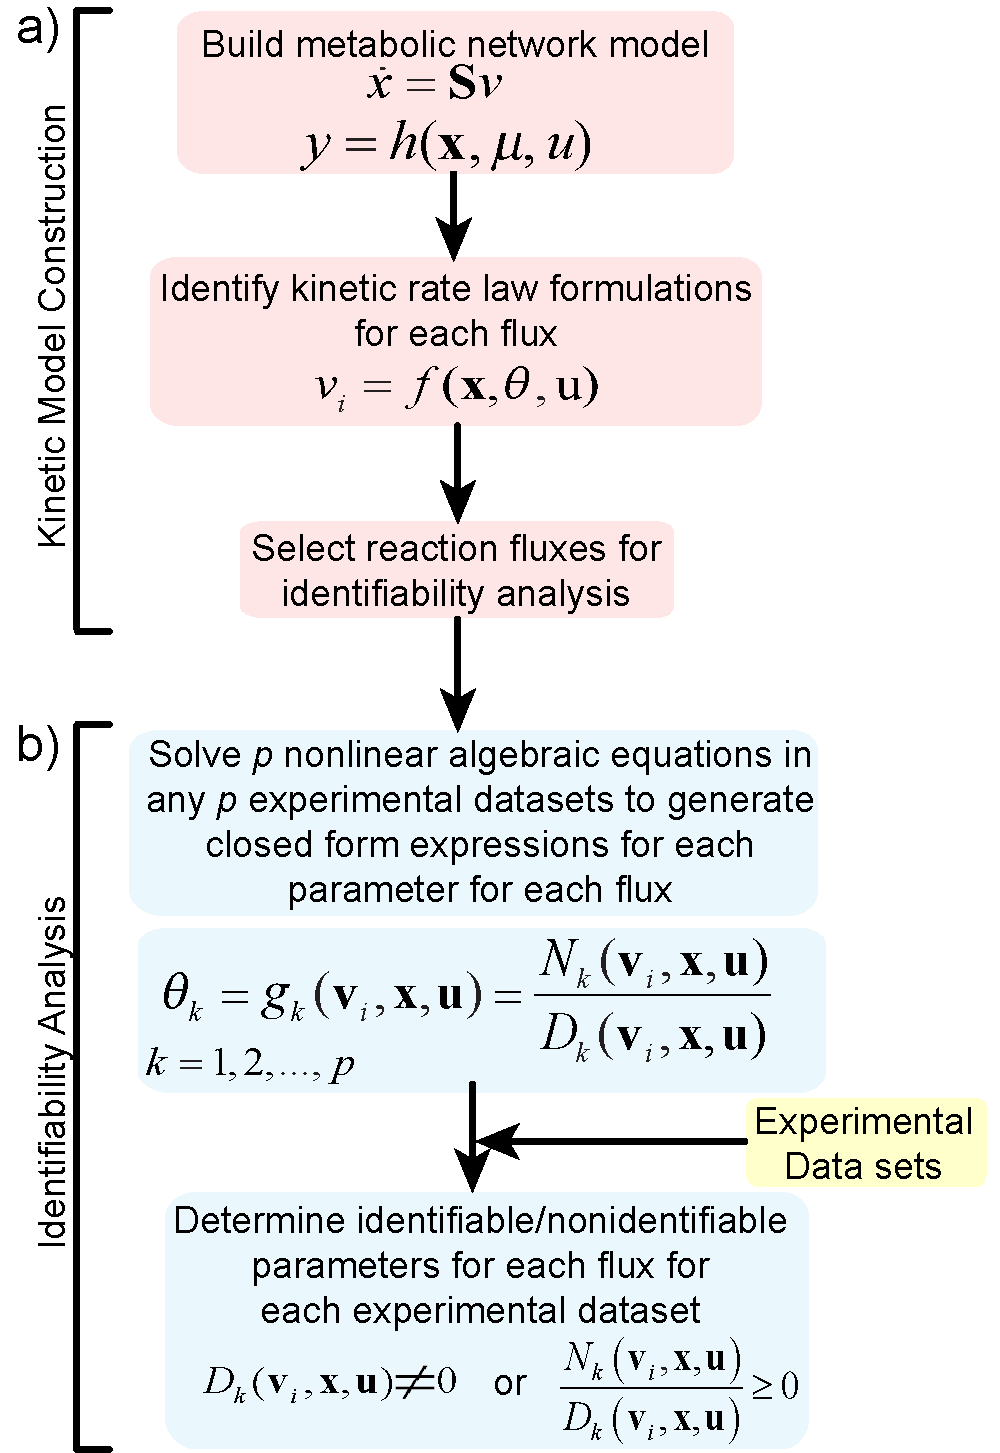
\includegraphics[width=.9\textwidth,height=.6\textheight,keepaspectratio]{figures/figure3/ident_analysis}}
		\caption{A flow diagram showing the methodology developed to establish practical identifiability of parameters in kinetic models of metabolism. a) The steps for the construction of a kinetic model of a metabolic network. The choice of rate law formulations to describe metabolic fluxes influences the identification methodology. The identifiability of parameters for each flux can be established independently. b) The steps for practical identifiability analysis for parameters of a single flux.}\label{fig:ident-flowchart}
	\end{figure}	
	
	The first step (Figure \ref{fig:ident-flowchart}a) involves the construction of the kinetic model (Equation \ref{eq:kinstoich}) of the metabolic network. For each flux $v_i$, $i={1, 2, ..., n_r}$, in the kinetic model, let $\mathbf{\theta} \in \mathbb{R}^{p}$ in Equation (\ref{eq:kinstoich}b). If data from $n_E$ experiments is available for the chosen metabolic network, as stated earlier, for each experiment $j = {1, 2, ..., n_E}$, we assume that all metabolite concentrations ($x\in\mathbb{R}^{n_x}$) and reaction fluxes ($v\in\mathbb{R}^{n_r}$) are measurable. We discuss the implications of relaxing this assumption in the results section. The pertinent information for each experiment $j$ is available as a vector of concentrations and fluxes, $\mathbf{x}_j$ and $\mathbf{v}_j$, respectively (Figure \ref{fig:ident-flowchart}b). 
	
	In order to establish the structural and practical identifiability of kinetic parameters for each flux $v_i$, $i={1, 2, ..., n_r}$, we describe a computer algebra-based method. The primary use of the computer algebra system is to obtain closed-form expressions for each parameter in $\mathbf{\theta} \in \mathbb{R}^p$ for each flux $v_i$ (Figure \ref{fig:ident-flowchart}b). This is done by first selecting a combination of $p\le n_E$ experiments. The fluxes and concentrations from these $p$ different experiments are then used to formulate a system of nonlinear algebraic equations in $\mathbb{R}^{p}$ for each flux $v_i$, as shown in Equation (\ref{eq:nonlineq}). 
	\begin{align}\label{eq:nonlineq}
	v_{i, j} = f_j(\mathbf{x}_j,\mathbf{\theta}, \mathbf{u}_j) && \forall j=\{1, 2, ..., p\}\subset\{1, 2, ..., n_E\}
	\end{align}
	Here, $v_{i,j}$ refers to the measured value of flux $v_i$ from experiment $j$. $\mathbf{x}_j$ and $\mathbf{u}_j$ are the vector of metabolite and other input concentrations from each experiment $j$, and $\mathbf{\theta}$ is a vector in $\mathbb{R}^{p}$, whose elements are denoted by $\theta_k$.		
	
	Each equation in (\ref{eq:nonlineq}), indicated by the index $j$, corresponds to the kinetic rate law expression $f(x, \theta, u)$ for each $v_i$, $i={1, 2, ..., n_r}$, described in Equation (\ref{eq:kinstoich}b), written for concentrations ($\mathbf{x}_j$, $\mathbf{u}_j$) and fluxes ($v_{i,j}$) obtained from experiment $j$. Solving the system in Equation (\ref{eq:nonlineq}) results in $\mathbb{R}^{p}$ nonlinear expressions for each parameter $\theta_k$ in $\theta \in \mathbb{R}^{p}$ (Equation \ref{eq:theta-eq}), where $N(\mathbf{v}_i, \mathbf{x}, \mathbf{u})$ is the numerator of $g$, and $D(\mathbf{v}_i, \mathbf{x}, \mathbf{u})$ is the denominator of $g$ (Figure \ref{fig:ident-flowchart}b). Note that $\mathbf{v}_i$, $\mathbf{x}$ and $\mathbf{u}$ are used to denote vector of vectors of fluxes for reaction $i$ ($\mathbf{v}_i$), metabolite ($\mathbf{x}$) and input ($\mathbf{u}$) concentrations, respectively, obtained from $p$ experiments, each denoted by the index $j = {1, 2, ..., p}$.
	\begin{align}\label{eq:theta-eq}
	\theta_k = g_k(\mathbf{v}_i, \mathbf{x}, \mathbf{u}) = \frac{N_k(\mathbf{v}_i, \mathbf{x}, \mathbf{u})}{D_k(\mathbf{v}_i, \mathbf{x}, \mathbf{u})}
	\end{align}
	
	Consistent with the definitions presented in Section \ref{sec:ident_def} above, we can define structural identifiability for a parameter $\theta_k$ as follows: if a unique solution (Equation \ref{eq:theta-eq}) exists for $\theta_k$, then $\theta_k$ is said to be structurally identifiable. However, if multiple finite solutions exists, then $\theta_k$ is only locally structurally identifiable. In the absence of any solution, $\theta_k$ is designated as a structurally non-identifiable parameter. 
	
	Similarly, any parameter $\theta_k$ is said to practically identifiable if the solution $g_k(\mathbf{v}_i, \mathbf{x}, \mathbf{u})$ in Equation (\ref{eq:theta-eq}) is unique for any given experimental data set. An infinite number of solutions are possible for a practically non-identifiable $\theta_k$ for a given experimental data set. However, if there are multiple but finite number of solutions $g_k(\mathbf{v}_i, \mathbf{x}, \mathbf{u})$ for the same set of experimental data, then the corresponding parameter $\theta_k$ is locally practically identifiable. 	
	
	The number of solutions, and consequently, the practically identifiability of a parameter from a given data set can also be constrained on the basis of the physiological relevance of the parameter estimate. We designate only parameters with unique physiologically relevant solutions $g_k(\mathbf{v}_i, \mathbf{x}, \mathbf{u})$ as practically identifiable (Figure \ref{fig:ident-flowchart}b). Parameters with multiple physiologically relevant solutions, or no physiologically relevant solution are designated as locally practically identifiable and practically non-identifiable parameters, respectively. For instance, since enzyme kinetic parameters represent metabolite-enzyme affinities to either the catalytic or the regulatory sites of an enzyme, we consider only non-zero positive parameter estimates to be physiologically relevant. Thus, parameters with multiple solutions ($g_k(\mathbf{v}_i, \mathbf{x}, \mathbf{u})$) can be still be designated as practically identifiable if there is only one unique positive (physiologically relevant) solution among the infinitely many solutions. 	
	
	Consequently, the enzyme kinetic model for each flux $v_i$ can be designated as structurally (or practically) identifiable if every parameter $\theta_k$, $\theta \in \mathbb{R}^{p}$, modeling flux $v_i$ is also structurally (or practically) identifiable. However, if at least one parameter $\theta_k$ for flux $v_i$ is either locally structurally (or practically) identifiable or non-identifiable, then the model for flux $v_i$ is also said to be locally structurally (or practically) identifiable or non-identifiable, respectively.	
	
	\subsection{Degree of identifiability: A quantitative measure of practical identifiability}\label{sec:degree_of_identifiability}
	We express the practical identifiability of kinetic parameters using a simple quantitative term called the degree of identifiability. We describe the degree of identifiability of any single parameter as the percentage of all data combinations (used to test for practical identifiability) that can identify that parameter. 
	
	As an example, if 90\% of all the experimental data combinations used for testing can identify a parameter $\theta_i$, then the degree of identifiability of $\theta_i$ is said to be 0.9 or 90\%. On the other hand, if only 10\% of the combinations can identify another parameter $\theta_j$, then $\theta_j$ has a degree of identifiability of 0.1 or 10\%. Furthermore, we can create a hierarchy of practically identifiable parameters using their degrees of identifiability. In the above instance of the two parameters $\theta_i$ and $\theta_j$ that have degrees of identifiability of 90\% and 10\% respectively, $\theta_i$ is classified to be more identifiable than $\theta_j$ due to its relatively higher degree of identifiability. 
	
	Determining this hierarchy of identifiable parameters can help in distinguishing parameters that can be identified by any type and any combination of experiments from parameters that can be identified by only a select type and combination of experiments. Such a classification can subsequently be used to design minimal sets of experiments that can practically identify all kinetic parameters used to model a metabolic network, going from the least identifiable parameter to the most identifiable parameter.  	
	
	\subsection{Experimental design through practical parameter identification}\label{sec:experimental_design}		
	Not all metabolite concentrations and fluxes in the model (Equation \ref{eq:kinstoich}) change for any random experiment. This makes unambiguous estimation of parameters impossible, either due to the inherent correlation between changes in different concentrations or fluxes, or due to the homeostasis of the concentrations and fluxes under the chosen experimental conditions \parencite{Heijnen2013}. In such scenarios, the need to design experiments to effect a change in, and discriminate between changes in different concentrations/fluxes becomes necessary. 
	
	Following the methodology described in Section \ref{sec:ident}, and demonstrated in Section \ref{sec:example} for a single flux using data from a combination of two different experiments, all distinct combinations of data sets obtained from experiments described in Section \ref{sec:experiments} of the Supplementary Information can be tested for their ability to practically identify any of the fluxes in the small metabolic network. This step would determine the degree of identifiability (defined in Section \ref{sec:degree_of_identifiability}) of each parameter in each flux in the model. 
	
	As mentioned in Section \ref{sec:ident}, the determination of practical identifiability of a parameter for a given set of experimental data requires determining the number and nature of possible solutions for each parameter $\theta_k$ in Equation (\ref{eq:theta-eq}). 
	The ability of a given set of experiments to satisfy conditions for practical identifiability can also be tested a priori without determining the number and nature of solutions $g_k(\mathbf{v}_i, \mathbf{x}, \mathbf{u})$ in Equation (\ref{eq:theta-eq}). This can be done by checking for the existence of solution $g_k(\mathbf{v}_i, \mathbf{x}, \mathbf{u})$, i.e., the value of $D_k(\mathbf{v}_i, \mathbf{x}, \mathbf{u})$ (Figure \ref{fig:ident-flowchart}b). Combinations of experiments for which the corresponding $D_k(\mathbf{v}_i, \mathbf{x}, \mathbf{u}) = 0$ can be designated as non-informative for practically identifying $\theta_k$. On the other hand, if $D_k(\mathbf{v}_i, \mathbf{x}, \mathbf{u})\neq0$, then the relevant experiments are informative, and can be used for determining practical identifiability. In summary, for practically identifiable parameters, the corresponding combinations of experiments should satisfy $D_k(\mathbf{v}_i, \mathbf{x}, \mathbf{u})\neq0$ and $g_k(\mathbf{v}_i, \mathbf{x}, \mathbf{u})$ should be unique and physiologically relevant. 
	
	We formally explain how the aforementioned criteria can be used to obtain a minimal and informative collection of experiments from which data can be used to identify and estimate as many model parameters as possible (Figure \ref{fig:ident-design}). The identifiability of each parameter based on each experiment with index $j = {1, 2, ..., n_E}$ is established based on the methodology summarized in Figure \ref{fig:ident-flowchart}b, and demonstrated in Section \ref{sec:example}. Subsequently, for any flux $v_i$, and for any combination of $p$ experimental data sets, if the experimental concentrations and fluxes ($\mathbf{x}_j$ and $\mathbf{v}_j$, respectively, where $j = {1, 2,..., p}$) do not satisfy the conditions for identifiability for any parameter $\theta_k$, $\theta\in\mathbb{R}^{p}$ (Figure \ref{fig:ident-flowchart}b), then at least one of the $p$ experiments needs to be replaced to make parameter $\theta_k$ identifiable. Consequently, the corresponding experiment cannot be used for estimating parameter $\theta_k$, and can be discarded from the set of all necessary experiments. Furthermore, another experiment from $j = {1, ..., n_E}$ needs to be selected to replace the discarded experiment such that parameter $\theta_k$ is identifiable. This process has to be repeated until all parameters in $\theta\in\mathbb{R}^p$ are identifiable for flux $v_i$. In doing so, we can arrive at a set of experiments that will always result in practically identifiable parameters for flux $v_i$. Note that if none of the $n_E$ pre-selected experiments satisfy the identifiability condition, then we can design an $(n_E+1)^{th}$ experiment that can replace one of the experiments that causes practical non-identifiability. This analysis can be performed for each flux in a metabolic network independent of all the other fluxes, making it theoretically scalable even to genome-scale models of metabolism. 		
	
	\subsection{Numerical parameter identification and estimation}\label{sec:numerical_method}
	The identification methodology described in the previous section can be extended to be used in conjunction with an optimization-based procedure for numerical estimation of parameters from experimental data. The $\mathbb{R}^p$ nonlinear algebraic equations formulated for each flux $v_i$ (Equation \ref{eq:nonlineq}) can be written as shown in Equation (\ref{eq:numerical_opt}) below to be solved as an optimization problem. Minimization of the sum of the absolute error values is used as the objective, and the $\mathbb{R}^p$ nonlinear algebraic equations are provided as inequality constraints. 
	
	\begin{subequations}\label{eq:numerical_opt}
		\begin{align}
		\underset{\theta, \varepsilon}{min} & \sum_{j=1}^{n_p} \left|\varepsilon_j\right|\\
		& v_{i, j} - f_j(\mathbf{x}_j,\mathbf{\theta}, \mathbf{u}_j) \le \varepsilon_j && j=\{1, 2, ..., n_p\}\\
		& \theta_l \le \theta_j \le \theta_u && j=\{1, 2, ..., n_p\}
		\end{align}
	\end{subequations}	
	
	Notice that the parameter values are bounded above and below by $\theta_u$ and $\theta_l$, respectively. These bounds can be specified to be arbitrarily large to include all possible parameter values.
		
	\subsection{Kinetic model of gluconeogenesis in \textit{E. coli}}\label{sec:small-model}
	A previously proposed kinetic model \parencite{Kotte2014, Srinivasan2017} for acetate consumption through gluconeogenesis (Figure \ref{fig:network}) is used as a case study to illustrate identifiability analysis for experimental design for parameter estimation in kinetic models of metabolism. The kinetic model is described below.
	
	\begin{figure}[!tbhp]
		\centering{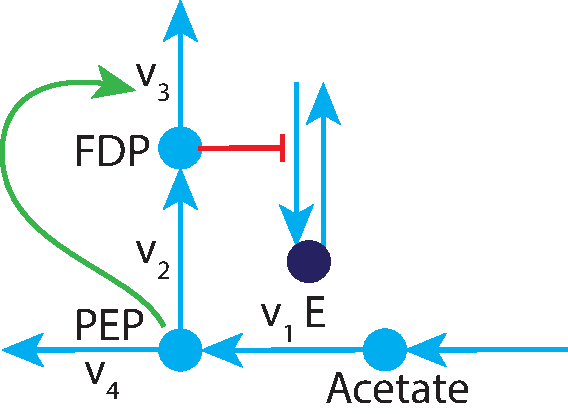
\includegraphics[width=.3\textwidth,height=.6\textheight,keepaspectratio]{figures/figure5/Figure1_NetworkA}}
		\caption{The previously published small metabolic network for gluconeogenesis used to demonstrate our practical identifiability method for kinetic models of metabolism.}\label{fig:network}
	\end{figure}		
	
	\begin{equation}\label{eq:ode1}
	\frac{d}{dt}pep=v_1-v_2-v_4
	\end{equation}
	\begin{equation}\label{eq:ode2}
	\frac{d}{dt}fdp=v_2-v_3
	\end{equation}
	\begin{equation}\label{eq:ode3}
	\frac{d}{dt}E=v_5 - d E
	\end{equation}
	The kinetic expressions for fluxes $v_1$ through $v_5$ are given below. The consumption of acetate through $v_1$ and conversion of \textit{pep} through $v_2$ are expressed in Equations (\ref{eq:flux1}) and (\ref{eq:flux2}) respectively using Michaelis-Menten kinetics. The acetate flux through $v_1$ is also governed by the quantity of available enzyme E. 
	\begin{equation}\label{eq:flux1}
	v_1 = k_{1}^{cat}E\frac{ac}{ac+K_{1}^{ac}}
	\end{equation}		
	The model for flux $v_1$ of the small network (Figure \ref{fig:network}), uses the concentration of the enzyme E as a variable (Equation \ref{eq:flux1}). Since we assume that steady state experimental information is only available for metabolite concentrations and fluxes, and not for enzyme concentration (again, the details on relaxing this assumption are discussed later), the expression in Equation (\ref{eq:flux1}) for $v_1$ cannot be used for identifying parameters $k_1^{cat}$ and $K_1^{ac}$. So, we modify the Michaelis-Menten kinetic rate law expression to eliminate the enzyme concentration E as a variable in Equation (\ref{eq:flux1a}). Consequently $k_1^{cat}$ is replaced by $V_1^{max}$ as a parameter to describe $v_1$. The corresponding enzyme binding constant is denoted as $K_1^{ac} (ne)$ to distinguish it from the enzyme binding constant calculated in the presence of measured enzyme concentration data.
	\begin{align}\label{eq:flux1a}
	v_1 = V_1^{max}\frac{ac}{ac+K_{1}^{ac}(ne)}
	\end{align}		
	We choose the expression for flux $v_1$ given in Equation (\ref{eq:flux1a}) to demonstrate our method for practical identifiability. 	
	\begin{equation}\label{eq:flux2}
	v_2 = V_{2}^{max}\frac{pep}{pep+K_{2}^{pep}}
	\end{equation}
	\begin{equation}\label{eq:flux3}
	v_3 = V_{3}^{max}\frac{\tilde{fdp}\left(1+\tilde{fdp}\right)^3}{\left(1+\tilde{fdp}\right)^4+L_3\left(1+\frac{pep}{K_{3}^{pep}}\right)^{-4}}
	\end{equation}
	The allosterically regulated flux $v_3$ for the consumption of \textit{fdp} is expressed in Equation (\ref{eq:flux3}) using the Monod-Wyman-Changeux (MWC) model for allosterically regulated enzymes, where $\tilde{fdp}$ refers to the ratio of \textit{fdp} with respect to its allosteric binding constant $K_{3}^{fdp}$. 
	
	The practically identifiability of parameters of a given flux are determined by solving a system of nonlinear algebraic equations using a computer algebra system (Section \ref{sec:ident}). We find that the nonlinearity of the MWC kinetic rate law used to model the allosteric regulation of $v_3$ makes it computationally intractable for determining the closed form expressions of the three parameters $V_3^{max}$, $K_3^{fdp}$ and $K_3^{pep}$ using a general purpose computer algebra system (Mathematica or SymPy in Python). We sought to overcome this computational obstacle by modeling flux $v_3$ using the convenience kinetic rate law \parencite{Liebermeister2006}. The corresponding expression for $v_3$ is given below (Equation \ref{eq:flux3_convkin}). 	
	\begin{align}\label{eq:flux3_convkin}
	v_3 = V_3^{max}\left(\frac{1}{1 + \frac{K_3^{pep}}{pep}}\right)\left(\frac{\frac{fdp}{K_3^{fdp}}}{1 + \frac{fdp}{K_3^{fdp}}}\right)
	\end{align}	
	
	The flux $v_4$ for the export of \textit{pep} is expressed as a linear equation dependent on $pep$ in Equation (\ref{eq:flux4}).
	\begin{equation}\label{eq:flux4}
	v_4 = V_{4}^{max}.pep
	\end{equation}		
	The production of enzyme E is represented by flux $v_5$. The inhibition of this flux by \textit{fdp} is modeled using Hill kinetics, where $K_e^{fdp}$ represents the Hill binding constant for the inhibiting metabolite \textit{fdp}, $n_e$ is the Hill exponent, and $V_e^{max}$ is the maximum reaction rate for $v_5$.
	\begin{align}\label{eq:flux5}
	v_5 = V_e^{max}\left(\frac{1}{1+\left(\frac{fdp}{K_{e}^{fdp}}\right)^{n_e}}\right)
	\end{align}
	
	\section{Results}
	First, in Section \ref{sec:example}, we demonstrate the use of the methodology that we described in Section 2.1 to practically identify parameters in flux $v_1$ of the small gluconeogenic network (Figure \ref{fig:network}) model given in Section \ref{sec:small-model}. 
	We discuss the ability of the proposed methodology to determine the structural identifiability of parameters modeling $v_1$, $v_3$ and $v_5$ in Section \ref{sec:proof}. 	
	In Section \ref{sec:initial_analysis} that follows, we show how the demonstrated methodology is capable of practically identifying and estimating parameters for fluxes $v_1$, $v_2$, $v_3$ and $v_5$ using steady state flux values and metabolite concentrations. 
	The various ways in which this information can be used for designing experiments to generate data that can facilitate estimation of identifiable parameters are discussed in Section \ref{sec:design}.
	The contribution of the uncertainty in the data arising from either the differences between in vivo and in vitro kinetics, or the noise present in experimentally measured quantities towards identifying parameters in enzyme kinetic models is discussed finally in Section \ref{sec:uncertainty}.
		
	\subsection{Identifying parameters in kinetic models of metabolism: an example}\label{sec:example}	
	We illustrate the proposed methodology, step by step, to identify parameters of flux $v_1$ in the small metabolic network (Figure \ref{fig:network} and Section \ref{sec:small-model}). We choose the expression for flux $v_1$ given in Equation (\ref{eq:flux1a}) for this demonstration. 
	
	Since $\theta = \{V_1^{max}, K_1^{ac} (ne)\} \in \mathbb{R}^2$ for $v_1$, as mentioned in Supplementary Section \ref{sec:experiments}, we need steady state concentration and flux measurements from at least two different experiments. So, from the $n_E = 21$ different experiments described in Supplementary Section \ref{sec:experiments} and Supplementary Table \ref{tab:pval}, we can choose multiple combinations of $p = 2$ experiments to satisfy the data requirements for identifying $v_1$ i.e., in Equation (\ref{eq:nonlineq}) $j = \{1, 2\}$. We label the available concentrations and fluxes as ${ac}^{(j)}$ and ${v_1}^{(j)}$, respectively. Then, the nonlinear algebraic equations shown in Equation (\ref{eq:nonlineq}) can be formulated for $v_1$ as:
	\begin{align*}%\label{eq:nonlin-flux2}
	{v_1}^{(j)} = V_{1}^{max}\frac{ac^{(j)}}{ac^{(j)}+K_{1}^{ac}(ne)} &&  j=\{1, 2\}
	\end{align*}
	
	Solving this simultaneous system of equations in $\mathbb{R}^2$ using Mathematica (Wolfram Research, USA), a general purpose computer algebra system, we get $p=2$ nonlinear algebraic expressions for parameters $V_1^{max}$ (Equation \ref{eq:v1_par}a) and $K_1^{ac}(ne)$ (Equation \ref{eq:v1_par}b). These expressions have the form shown in Equation (\ref{eq:theta-eq}).
	\begin{subequations}\label{eq:v1_par}
		\begin{align}		
		\theta_1 &= V_1^{max} = \frac{v_1^{(1)}v_1^{(2)}(ac^{(1)}-ac^{(2)})}{v_1^{(2)}ac^{(1)}-v_1^{(1)}ac^{(2)}}\\
		\theta_2 &= K_1^{ac}(ne) = \frac{ac^{(1)}ac^{(2)}(v_1^{(1)}-v_1^{(2)})}{v_1^{(2)}ac^{(1)}-v_1^{(1)}ac^{(2)}}
		\end{align}
	\end{subequations}
	The presence of a single unique expression for both $V_1^{max}$ and $K_1^{ac} (ne)$ shown above indicates that these parameters are structurally identifiable. 

	As described in Section \ref{sec:ident}, we use multiple combinations of in silico experimental data with Equation \ref{eq:v1_par} to assess the practical identifiability of $V_1^{max}$ and $K_1^{ac} (ne)$. First we determine the value of the denominator of the right hand side expression in Equation (\ref{eq:v1_par}). A non-zero value could potentially indicate an identifiable parameter. In addition, since the enzyme binding constant ($K_1^{ac}(ne)$) and the maximum reaction rate ($V_1^{max}$) cannot be negative, the values obtained from Equation (\ref{eq:v1_par}) should also be positive for these parameters to be classified as practically identifiable (Figure \ref{fig:ident-flowchart}b). All estimates for $V_1^{max}$ and $K_1^{ac} (ne)$ from all (240) possible combinations of experimental data are shown in Supplementary Figure \ref{fig:v1_v1max_ck_values}. Due to the numerous possible estimates for both parameters (Supplementary Figure \ref{fig:v1_v1max_ck_values}), we can conclude that they are practically non-identifiable. 
	
	So far, we have assumed that only information on metabolite concentrations and metabolic fluxes is available in the form of omics data sets. However, protein concentration measurements can also be obtained along with measured metabolite concentrations and fluxes. To ascertain the impact of such a scenario on parameter identifiability, we demonstrate the proposed methodology for identifying flux $v_1$ when it is modeled by Equation (\ref{eq:flux1}), and the practical identifiability is assessed in the presence of concentration measurements for the enzyme \textit{E}. Note that the parameter $V_1^{max}$ in Equation (\ref{eq:flux1a}) is substituted with $V_1^{max} = k_1^{cat}E$ in Equation (\ref{eq:flux1}), and the dimension of the parameter space for $v_1$ is still $\mathbb{R}^2$. The corresponding identifiability expressions for $k_1^{cat}$ and $K_1^{ac}$ are given in Equation (\ref{eq:v1_k1cat}) below.	
	\begin{subequations}\label{eq:v1_k1cat}
		\begin{align}
		k_1^{cat} = \frac{ v_1^{(1)}v_1^{(2)} \left( ac^{(1)}- ac^{(2)}\right)}{v_1^{(2)}ac^{(1)}E^{(1)} - v_1^{(1)}ac^{(2)}E^{(2)}}\\
		K_1^{ac} = \frac{ac^{(1)}ac^{(2)}\left(v_1^{(1)}E^{(2)} - v_1^{(2)}E^{(1)}\right)}{v_1^{(2)}ac^{(1)}E^{(1)} - v_1^{(1)}ac^{(2)}E^{(2)}}
		\end{align}
	\end{subequations}		
	This establishes the structural identifiability of the parameters.

	Following the procedure described in Section \ref{sec:ident} and demonstrated above for $V_1^{max}$, we are able to show that both $k_1^{cat}$ and $K_1^{ac}$ have unique estimates (Figure \ref{fig:ident_values}a), and are hence practically identifiable. Accordingly, we can summarize that the practical non-identifiability of $v_1$ (due to the uncertainty in the estimates of $V_1^{max}$ and $K_1^{ac}$ seen in Supplementary Figure \ref{fig:v1_v1max_ck_values}) can be mitigated through the incorporation of additional experimental data combined with a finer resolution of the model parameters. In this instance, the additional data takes the form of enzyme concentrations. 
	
	\begin{figure}[!tbhp]
		\centering{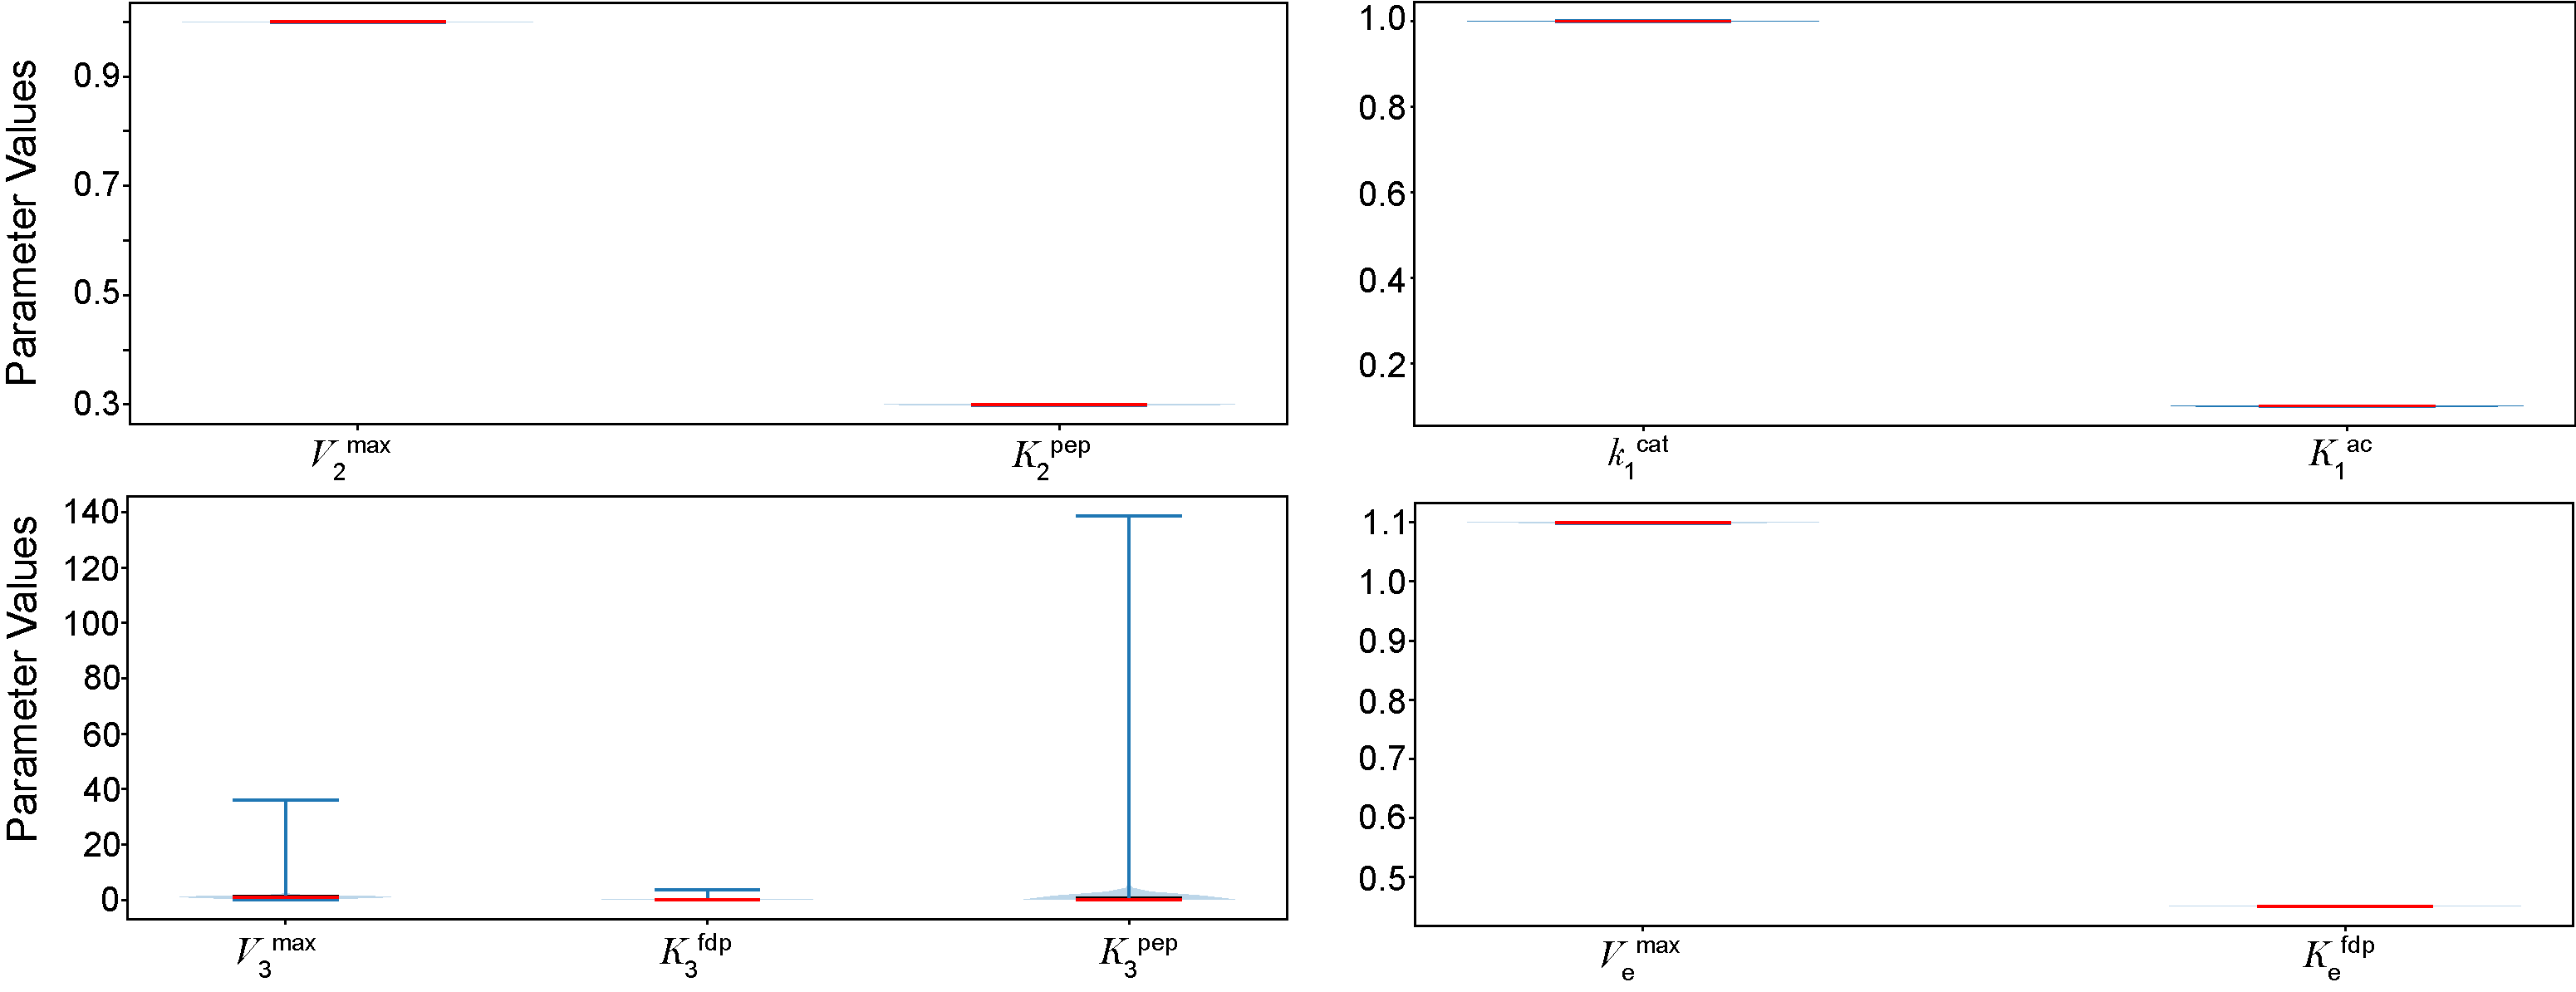
\includegraphics[width=1.0\textwidth,height=.8\textheight,keepaspectratio]{figures/parameter_dist/v1_kcat_v2_v5_2_v3_1_parameter_dist}}
		\caption{Distribution of predicted parameter values when performing practical identifiability analysis using closed-form solutions for each parameter in flux a) $v_1$, b) $v_2$, c) $v_5$, and d)$v_3$. For $v_1$, we have assumed that enzyme concentration is available and have accordingly identified and estimated $k_1^{cat}$, as opposed to $V_1^{max}$. The parameter values for only the second root of $K_e^{fdp}$ in $v_5$ ($K_e^{fdp}(2)$) is shown, since $K_e^{fdp}(1)$ is not estimated by any combination of two experiments, and $V_e^{max}$ is estimated by all combinations. Only one of the two roots for $v_3$ is shown in panel d. The estimated data for the second root has a similar distribution to that of the first root. Data is generated using the Convenience Kinetic model for allosteric regulation for  $v_3$.}\label{fig:ident_values}
	\end{figure}
	
	\subsection{Establishing structural identifiability of parameters based on closed-form solutions}\label{sec:proof}
	Here, we discuss results from the identifiability analysis of fluxes $v_2$, $v_3$ and $v_5$ in the small metabolic network (Figure \ref{fig:network}), using the methodology (Figure \ref{fig:ident-flowchart}) that we have demonstrated above for flux $v_1$
	
	In order to assess the identifiability of each flux in a metabolic network, we demonstrated in Section \ref{sec:example} that it should be possible to obtain closed form solutions (Equation \ref{eq:theta-eq}) for each parameter in the enzyme kinetic model for each flux (Figure \ref{fig:ident-flowchart}). Subsequently, we also illustrated the ability to establish structural identifiability based on the number of closed-form solutions obtained for each parameter by using flux $v_1$ as an example (Section \ref{sec:example}). Recall that flux $v_1$, in both forms (Equations \ref{eq:flux1} and \ref{eq:flux1a}), is expressed as a Michaelis-Menten model. Hence, by extension, we can conclude that $v_2$, which is also modeled as Michaelis-Menten flux, is also structurally identifiable with unique expressions for $V_2^{max}$ and $K_2^{pep}$. The closed-form expressions for these parameters are similar to the ones shown in Equation \ref{eq:v1_par}, with \textit{ac} replaced by \textit{pep}, and $v_1$ replaced by $v_2$. 
	However, we find that Convenience kinetics rate law model for $v_3$ (Equation \ref{eq:flux3_convkin}), and Hill kinetic rate law model for $v_5$ (Equation \ref{eq:flux5}) are not structurally identifiable.
	
	In the case of $v_3$, we find that the parameters $V_3^{max}$, $K_3^{fdp}$ and $K_3^{pep}$ have non-unique but a finite number of solutions, i.e., we get two distinct solutions for each parameter. So, $v_3$ is only locally structurally identifiable. We tried establishing global structural identifiability by reducing the dimension of the parameter space $\theta$ for $v_3$ from $\mathbb{R}^3$ to $\mathbb{R}^2$. We do so by fixing either $K_3^{fdp}$ or $K_3^{pep}$ as a known quantity, and identify the other unfixed parameter along with $V_3^{max}$. This results in unique expressions for both $V_3^{max}$ and the other unfixed parameter ($K_3^{pep}$ or $K_3^{fdp}$). Thus, by reducing the dimension of $\theta$ to $\mathbb{R}^2$, we were able to obtain a structurally identifiable model for $v_3$.  
	
	Next, we describe results obtained in determining the identifiability of $v_5$, which describes a transcription/translation reaction using Hill kinetics (Equation \ref{eq:flux5}), using only the available experimental data on the metabolite concentrations and the fluxes within the metabolic network. 	
	Recall that we use the Convenience kinetic model as opposed to the MWC model for $v_3$ due to the inability of the computer algebra system to solve for the parameters in the MWC model. Similarly, for $v_5$, the computer algebra system could not solve for all three model parameters: $V_e^{max}$, $K_e^{fdp}$ and $n_e$. So, instead changing the model (as in $v_3$), we resorted to reducing the dimension of the parameter space by fixing one of the three parameters, the Hill coefficient $n_e$. With a fixed and known $n_e$, $K_e^{fdp}$ has two possible solutions, and $V_e^{max}$ has only one unique solution. Thus, $v_5$ is locally structurally identifiable. 
	
	Thus, in the process of establishing the structural identifiability of $v_3$ and $v_5$ we have shown that our methodology is capable of extracting the existence of meaningful relationships between different enzyme kinetic parameters using only steady state concentrations and fluxes. We have also shown how the existence of these relationships affects the structural identifiability of the enzyme kinetic models for $v_3$ and $v_5$, and under what conditions these relationships can be removed to make some of the most prevalent enzyme kinetic models structurally identifiable. 	
	
	\subsection{Relationship between structural and practical parameter identifiability}\label{sec:initial_analysis}
	Having established conditions for structural identifiability of fluxes $v_1$, $v_2$, $v_3$ and $v_5$ in the previous sections, we look at the practical identifiability of these flux models, and the impact that it has on the choice of experiments chosen to estimate the parameters in these models.	
	
	We find that both $v_1$ and $v_2$, which are structurally identifiable (Section \ref{sec:proof}), are also practically identifiable. The parameters in the respective models possess unique values based on distinct combinations of experimental data (Figure \ref{fig:ident_values}a and b and Supplementary Figures \ref{fig:v1_kcat_ck_values} and \ref{fig:v2_ck_values}). 
	
	It is well understood in the systems identification community that structural identifiability is a necessary condition for practical identifiability (). So, in the case of $v_3$, which is only locally structurally identifiable, we would expect it to at least be locally practically identifiable. However, we not only find that the parameter estimates for $V_3^{max}$, $K_3^{fdp}$ and $K_3^{pep}$ in the Convenience kinetics model for $v_3$ are not unique (Figure \ref{fig:ident_values}c), we also observe large uncertainties in these estimates (Figure \ref{fig:ident_values}c and Supplementary Figure \ref{fig:v3_ck_values}).  These observations lead us to conclude that when using steady state data to establish practical identifiability, the local structural identifiability of $v_3$ does not guarantee its practical identifiability, local or otherwise. 
	
	However, we find $v_3$ to be practically identifiable when its parameters are also structurally identifiable (Figure \ref{fig:v3_var_ck_values}). Earlier in Section \ref{sec:proof} we had mentioned that $V_3^{max}$ and $K_3^{fdp}$ are structurally identifiable only when the dimension of the parameter space is $\mathbb{R}^2$, and not in $\mathbb{R}^3$, i.e., either $K_3^{pep}$ of $K_3^{fdp}$ is fixed to identify $V_3^{max}$ and the other enzyme affinity constant. Under these scenarios we find both parameters in $\mathbb{R}^2$ to be structurally and practically identifiable (Figure \ref{fig:v3_var_ck_values}).	
	
	\begin{figure}[!tbhp]
		\centering{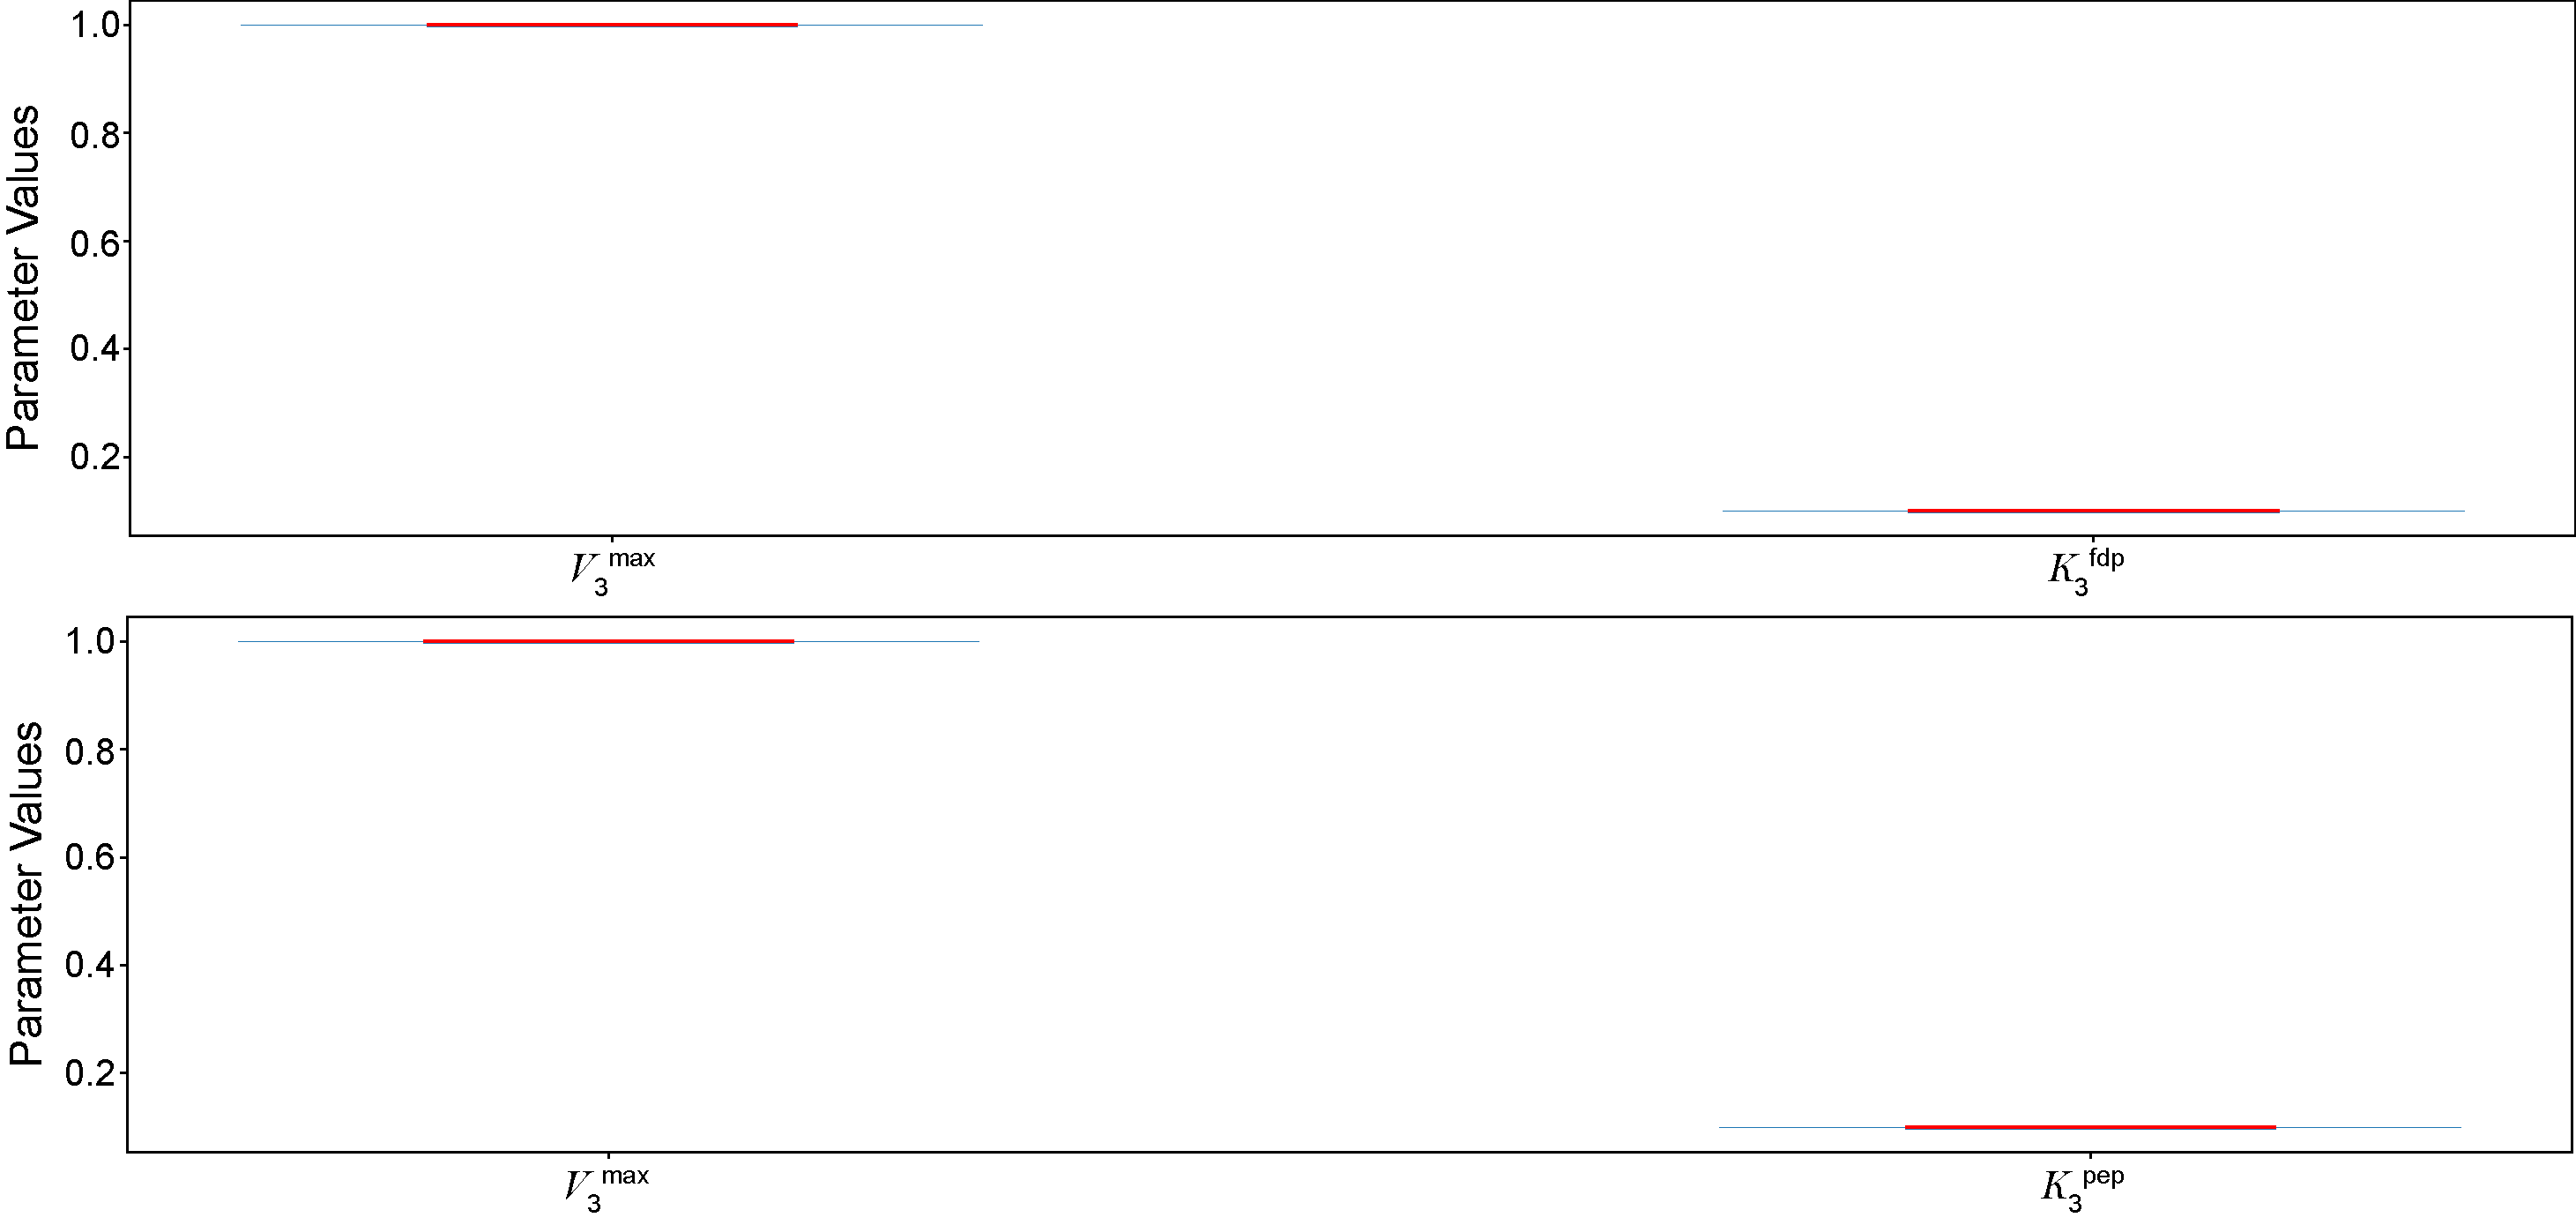
\includegraphics[width=0.8\textwidth,height=0.8\textheight, keepaspectratio]{figures/parameter_dist/v3_var_parameter_dist}}
		\caption{Distribution of predicted parameter values when performing practical identifiability analysis using closed-form solutions for each parameter in flux $v_3$. The globally identifiable parameter values of a)  $V_3^{max}$ and $K_3^{fdp}$ when $K_3^{pep}$ is held constant, and b) $V_3^{max}$ and $K_3^{pep}$ when $K_3^{fdp}$ is held constant.}\label{fig:v3_var_ck_values}
	\end{figure}	
	
	Regarding $v_5$, we showed earlier in Section \ref{sec:proof} that $v_5$ is structurally identifiable only when the Hill coefficient $n_e$ is held constant. Given the need for structural identifiability to study practically identifiability, in subsequent discussions, the dimension of the $v_5$ parameter space is kept at $\mathbb{R}^2$ by fixing the value of $n_e$. Under these conditions, we find $V_e^{max}$ to be both structurally and practically identifiable (Figure \ref{fig:ident_values}d and Supplementary Figure \ref{fig:v5_ck_values}). However, recall from Section \ref{sec:proof} that unlike $V_e^{max}$, $K_e^{fdp}$ is only locally structurally identifiable as it has two possible closed-form expressions. Nonetheless, despite its local structural identifiability, we find that the $K_e^{fdp}$ is also practically identifiable, like $V_e^{max}$, with only one unique parameter value (Figure \ref{fig:ident_values}d and Supplementary Figure \ref{fig:v5_ck_values}). Thus, $v_5$ is practically identifiable despite its local structural identifiability. This can primarily be attributed to the enforcement of the physiological relevance criteria on the parameters i.e., only one of the two closed-form expressions for $K_e^{fdp}$ is physiologically relevant for all available experimental data sets.
	 The other solution always acquires a negative value that has no physiological meaning. Thus, by reducing the practically identifiable space of parameters, we have shown that our methodology can establish global practical identifiability even when the parameters are only locally structurally identifiable, again using only steady state experimental data. 
	 
	 To summarize, $v_3$ in practically non-identifiable when it is only locally structurally identifiable. In contrast, $v_5$ is practically identifiable even in the presence of local structural identifiability. Hence, using $v_3$ and $v_5$ as examples we have shown that in using steady state data to determine both structural and practical identifiability in kinetic models of metabolism, it is possible to establish a relationship between structural and practical identifiability only under certain conditions, and not in others.	 
	
	\subsection{A priori experimental design through practical parameter identification}\label{sec:design}	
	In Section \ref{sec:experimental_design} and Figure \ref{fig:ident-flowchart}b we describe how the analysis of practical identifiability of a parameter can be used to gather information on the type of experiments that can provide useful data for parameter estimation. In Section \ref{sec:degree_of_identifiability}, we also describe how this analysis allows us to arrange parameters hierarchically on the basis of their degree of identifiability. In this section we show how these two methods combined can be used to design experiments to provide informative data for parameter estimation in the kinetic model of small metabolic network (Figure \ref{fig:network}).
	
	\begin{figure}[!tbhp]
		\centering{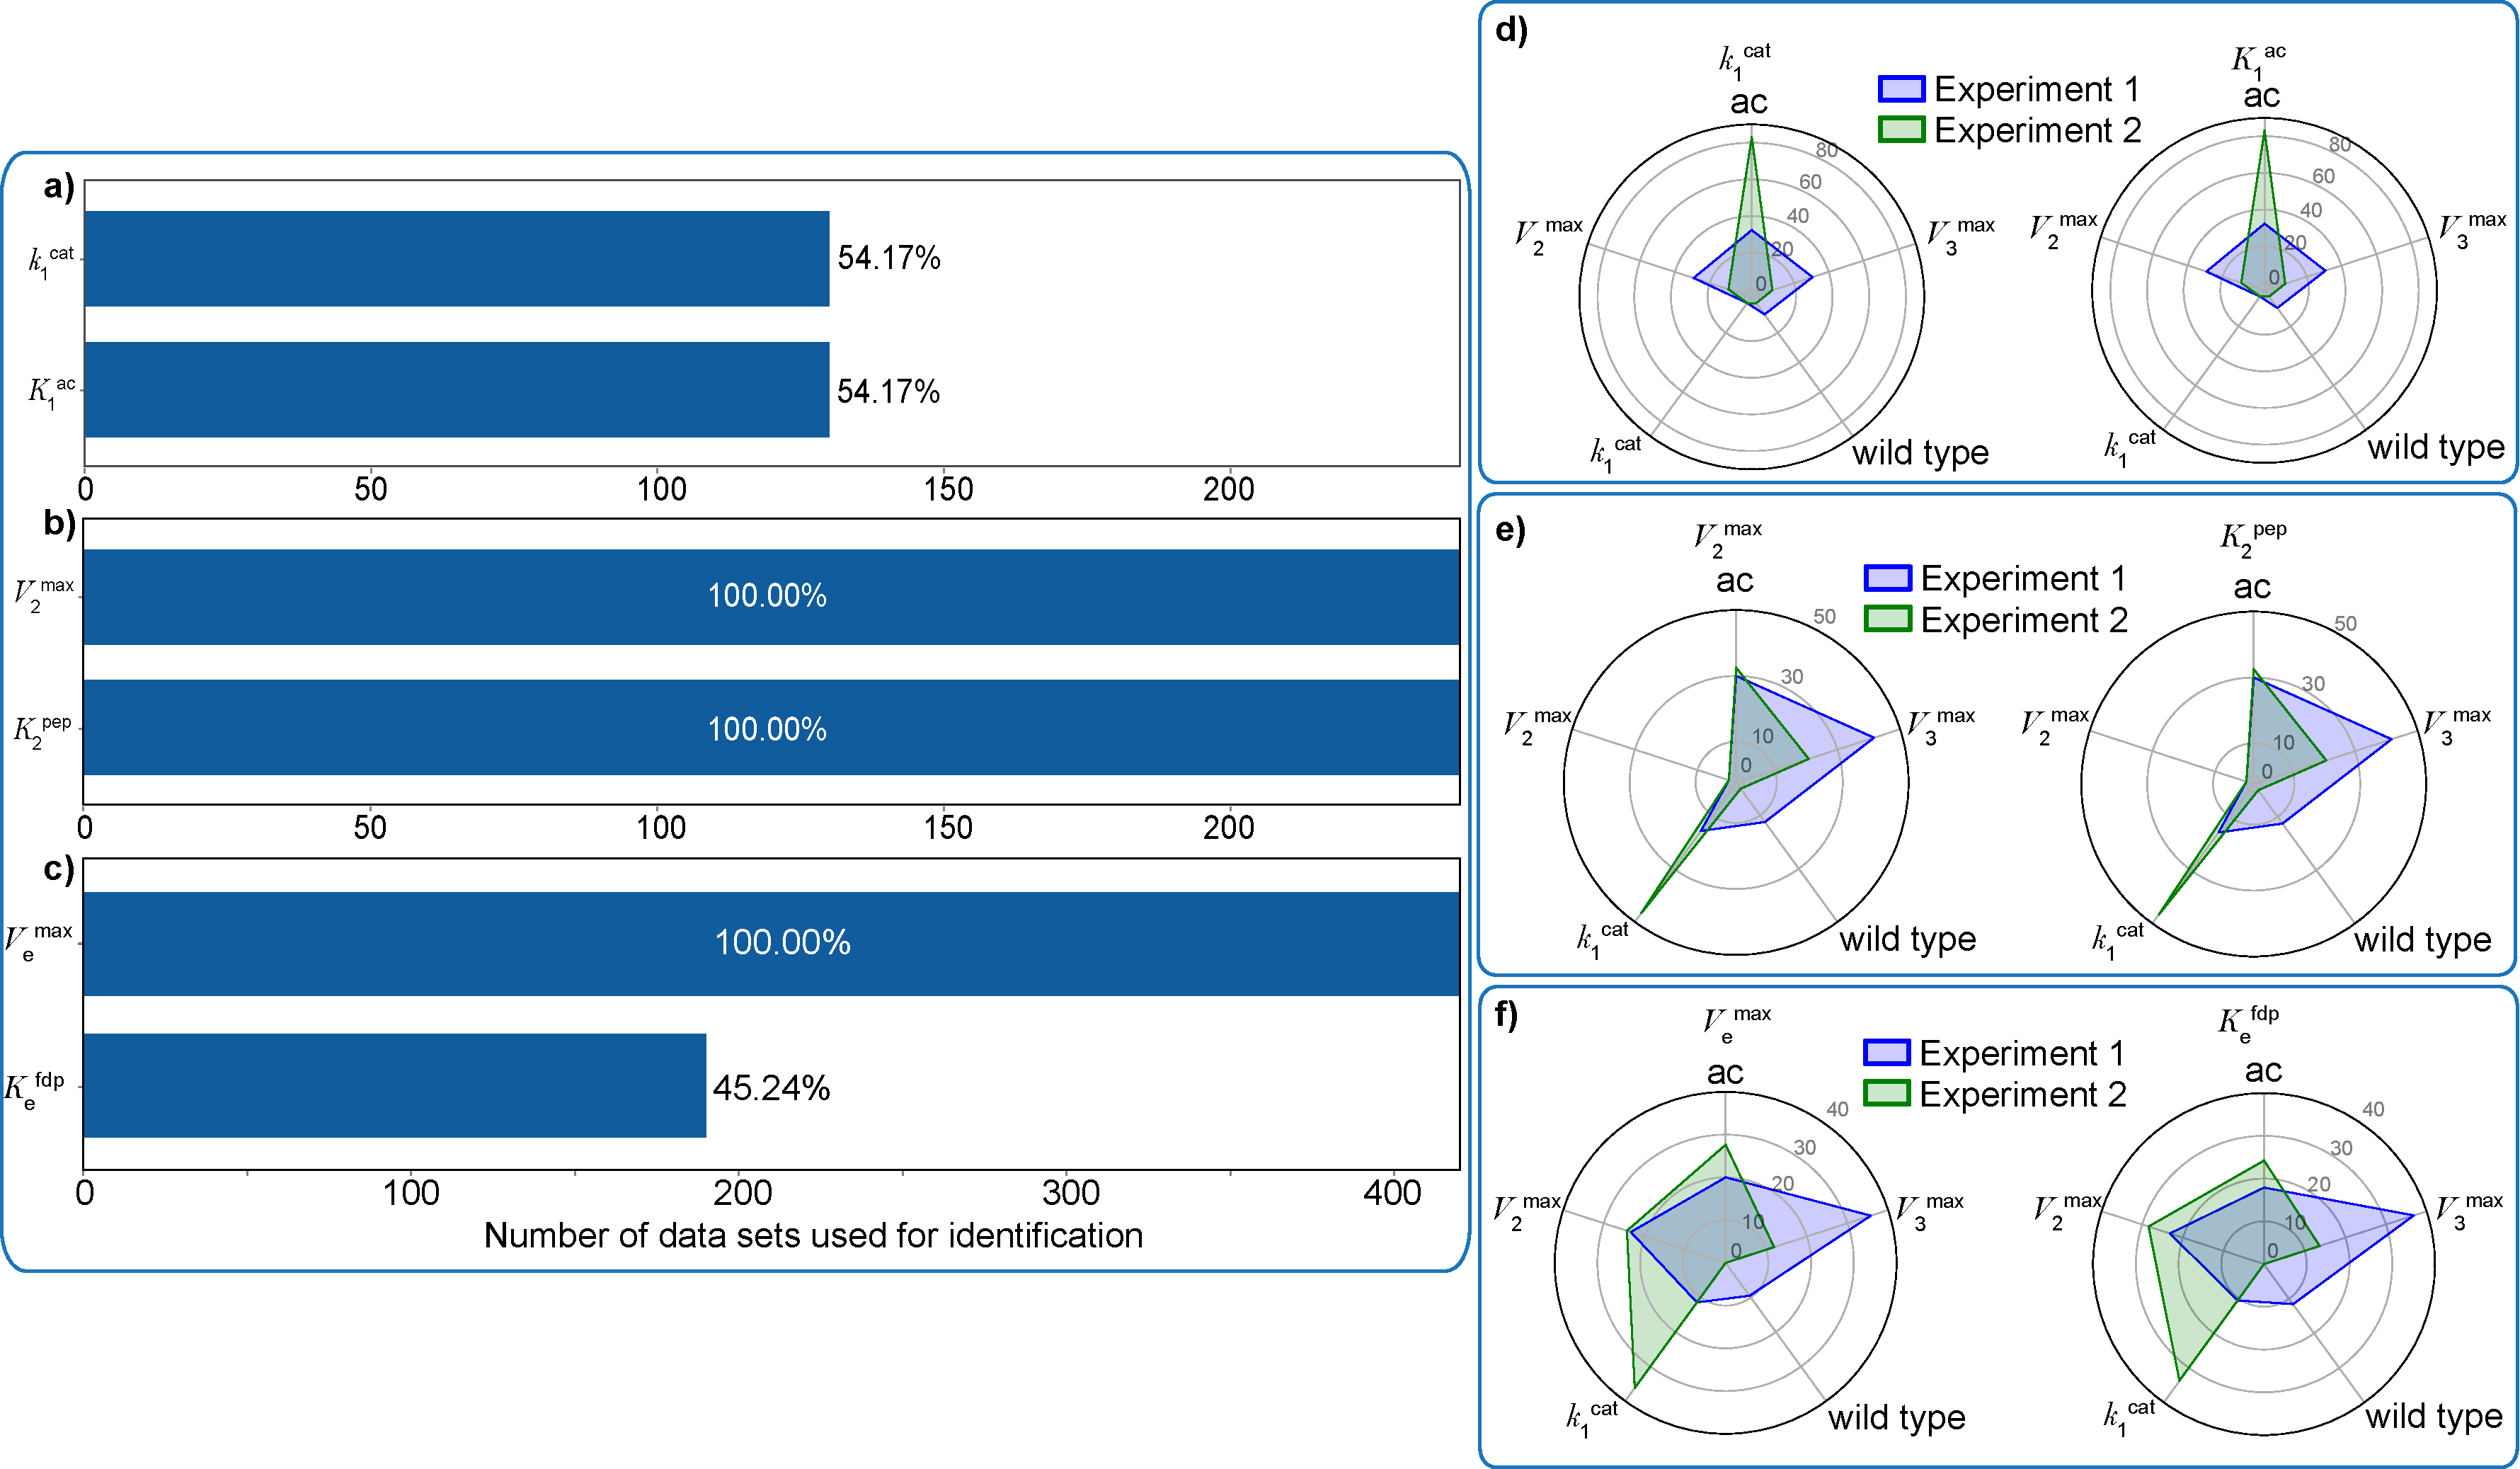
\includegraphics[width=1.0\textwidth,height=0.9\textheight,keepaspectratio]{figures/ident_exp_info/v1_kcat_v2_v5_2_exp_info}}
		\caption{The number of data combination from 21 different in silico experiments that can practically identify each parameter in fluxes a) $v_1$, b) $v_2$, and c) $v_5$ when there is no noise in the input experimental data. The percentage of total combinations of experimental data used for analysis (240 for $v_1$ and $v_2$, and 421 for $v_5$) that can identify each parameter is also specified. $v_1$, $v_2$ and $v_5$ require data from two experiments for analysis. The contribution of different experiment type towards identifying each parameter is shown in the spider plots for d) $v_1$, e) $v_2$ and f) $v_5$. The choice of perturbation chosen for the first experiment (blue) determines the choice of the second perturbation (green) required for identifying the parameters.}\label{fig:ident}
	\end{figure}
	
	In Figure \ref{fig:ident}a-c we show the degree of identifiability (percentage of experimental data combinations that are capable of identifying each parameter) of each parameter in each of three fluxes $v_1$, $v_2$ and $v_5$, respectively. The degree of identifiability of $v_1$ based on Equation (\ref{eq:flux1a}) is provided in Supplementary Figure \ref{fig:v1_v1max_ck_ident}. Note that we perform this analysis only for conditions under which the structural and practical identifiability of these fluxes can be established without doubt. So, based on the small uncertainties observed for $V_1^{max}$ and $K_1^{ac} (ne)$ (Supplementary Figure \ref{fig:v1_v1max_ck_values}), we classify the corresponding model of $v_1$ (Equation \ref{eq:flux1a}) as locally practically identifiable. Although, this analysis can be performed for fluxes that are not practically identifiable, i.e., $v_3$, we doubt the meaningfulness of such an analysis (Supplementary Figure \ref{fig:v3_1_ck_ident}). It is important to note that in scenarios where fluxes are only locally practically identifiable the degree of identifiability (Supplementary Figure \ref{fig:v1_v1max_ck_ident} for $v_1$ and Supplementary Figure \ref{fig:v3_1_ck_ident} for $v_3$) refers to the number of experimental data sets that can determine physiologically relevant values for the corresponding parameters.
	
	First, we see that the maximum reaction rates ($V_i^{max}$) are more or similarly identifiable in comparison to the corresponding enzyme binding ($K_i$) constants or the activation/inhibition constants, in the respective reaction rate law models (Figure \ref{fig:ident}, Supplementary Figures \ref{fig:v1_v1max_ck_ident} and \ref{fig:v3_1_ck_ident}). This is true despite the fact that the different fluxes are modeled using different enzyme kinetic rate laws: $v_1$ and $v_2$ are modeled using the Michaelis-Menten rate law, $v_3$ is modeled using the Convenience kinetic rate law and $v_5$ is modeled as a Hill equation with inhibition.
	
	The degree of identifiability of parameters in $v_3$, when it is structurally and practically identifiable (Sections \ref{sec:proof} and \ref{sec:initial_analysis}) is shown in Supplementary Figure \ref{fig:v3_var_1_2_ck_ident}. In conjunction with the degree of identifiability of other parameters (Figures \ref{fig:ident} and Supplementary Figure \ref{fig:v1_v1max_ck_ident}), we find that with the exception of $V_1^{max}$ (Supplementary Figure \ref{fig:v1_v1max_ck_ident}) and $k_1^{cat}$ in $v_1$ (Figure \ref{fig:ident}a), all data sets used to test practical identifiability can determine unique values for parameters when the corresponding parameter is structurally identifiable. 	
	
	We can attribute the difference in the degree of identifiability between $v_1$ (Figure \ref{fig:ident}a and Supplementary Figure \ref{fig:v1_v1max_ck_ident}) and the other fluxes ($v_2$, $v_3$ and $v_5$) to the ability of data from different combinations of experiments to satisfy the conditions for practical identifiability of that parameter. In systems identification terminology, data requirements for parameter identification can be tied to selecting experiments that are persistently excitable for the flux being identified. Any input signal should be rich or informative enough to guarantee full excitement of the dynamics of the system \parencite{Ljung1994}. Only information obtained from such changes in the input can be used to completely identify the system over its entire dynamic range. So, the ability of data from a combination of different experiments to practically identify parameters of a given flux is governed by the ability of the experiment to generate distinct measured concentrations and fluxes that will satisfy the identifiability conditions. 	
	
	In turn, the degree of identifiability of parameters and the informativeness of the corresponding experiments used to identify them can be explained by the position of the flux in the metabolic network. The position of any given flux in the metabolic network determines the specific experiment that is persistently excitable enough to identify the parameters of that flux. This dependency can be further elucidated using $v_1$ and $v_2$ as examples. 
	
	We know from Equation (\ref{eq:v1_k1cat}) and Section \ref{sec:example} that for a combination of any two experiments to be capable of identifying $v_1$, the experiments must generate data that have distinct acetate concentrations, \textit{E} and $v_1$. We also know, based on our knowledge of the Michaelis-Menten kinetic rate law that changes in the substrate concentration of a reaction can bring about a nonlinear change in the value of the corresponding reaction rate. So, in this instance, since the substrate is an input variable to the model, and $v_1$ is the corresponding uptake flux and \textit{E} is a system variable, the substrate can be easily perturbed to create persistently excitable experiments to identify parameters in $v_1$. We see the consequence of this requirement in the degree of identifiability of $k_1^{cat}$ and $K_1^{ac}$ (Figure \ref{fig:ident}a). We can generalize this observation for the identification of all uptake fluxes in all metabolic networks, i.e., at a minimum, a change in the input substrate concentration may be necessary for an informative experiment to identify the uptake flux parameters. 
	
	Similarly, the identification of parameters for $v_2$ (Figure \ref{fig:ident}b) requires that persistently excitable experiments distinguish between values of both $v_2$ as well as \textit{pep}. However, since both of these are system outputs, satisfaction of this condition cannot be guaranteed without an analysis of the dynamics of the metabolic network, and how changes in the input (acetate) bring about changes in the two requisite output quantities. Previous dynamical analysis of the network (Figure \ref{fig:network}) has already established the existence of a functional relationship between \textit{pep} and $v_2$, and the input acetate concentration and the levels of expression of the different enzymes within the network \parencite{Srinivasan2017}. The 100\% degree of identifiability seen for $v_2$ (Figure \ref{fig:ident}b) confirms the theoretical possibility for any type of perturbation experiment to be persistently excitable to identify $v_2$. Overall, this analysis informs us that the degree of identifiability and consequently, the type of experiments needed to identify different parameters varies widely depending on the position of the flux with respect to the inputs and the outputs of the metabolic network, as well as the various regulatory interactions present within the network (e.g., effect of \textit{pep} on $v_3$, or the effect of \textit{fdp} on $v_5$ and consequently on $v_1$ in Figure \ref{fig:network}). 	
	
	From the above example we can summarize that identification of individual fluxes within a metabolic network necessitates a careful consideration of experiments such that the data acquired can satisfy conditions for practical identifiability for all parameters modeling a flux, and subsequently, all fluxes within a network \parencite{Heijnen2013}. 
	
	To facilitate the design of experiments based on their ability to satisfy requirements for practical identifiability of parameters, we determine the occurrence of each type of steady state perturbation experiment within combinations that can practically identify each parameter (Figure \ref{fig:ident}d-f, Supplementary Figures \ref{fig:v1_v1max_ck_ident},  \ref{fig:v3_1_ck_ident} and \ref{fig:v3_var_1_2_ck_ident}). So, with our proposed methodology it is possible to identify the types of perturbation experiments that would be informative for identifying each parameter in each flux with steady state concentration and flux data. In these figures the contribution from different experiment types for identifying parameters in $v_1$, $v_2$ and $v_5$ are respectively shown as spider plots. 
	
	The contribution of experiments that involve changes in the acetate concentrations, which consequently bring about changes in the value of $v_1$, contribute to a significant part ($\approx$80\%) of the identifiable experimental data combinations for $v_1$ in comparison to the other types of experiments (Figure \ref{fig:ident}d and Supplementary Figure \ref{fig:v1_v1max_ck_ident}). This is in agreement with the condition for identifiability that we discussed earlier and showed mathematically (Equations \ref{eq:v1_k1cat} and \ref{eq:v1_par}). Since only about 50\% of all data combinations can satisfy these requirements, and can consequently identify $v_1$ (Figure \ref{fig:ident}a), we also say that identifiability analysis is crucial to determine the minimum number of experiments, along with the nature of experiments that can help identify parameters for $v_1$. 
	
	With $v_2$, we see that the enzyme perturbations as well as the acetate perturbation experiments have similar contributions towards datasets that can identify $v_2$ (Figure \ref{fig:ident}e). This also supports our arguments made earlier with regards to the identifiability conditions for $v_2$, and the reasons for the difference in the type of experiments that are informative between $v_1$ and $v_2$. Accordingly, we find that in comparison to selecting experiments to identify $v_1$, there is very little restriction on the types of experiments that are informative to identify $v_2$.
	
	We can also extend these observations to justify the observed contribution of experiments towards identifying parameters for $v_5$ (Figure \ref{fig:ident}f), or determining physiologically relevant parameter values for structurally locally identifiable parameters of $v_3$ (Supplementary Figures \ref{fig:v3_1_ck_ident} and \ref{fig:v3_var_1_2_ck_ident}). 
	
	In all of the above scenarios for $v_1$ (Figure \ref{fig:ident}d), $v_2$ (Figure \ref{fig:ident}e), $v_3$ (Supplementary Figures \ref{fig:v3_1_ck_ident} and \ref{fig:v3_var_1_2_ck_ident}) and $v_5$ (Figure \ref{fig:ident}f), the distribution of experiment types between second, and in the case of $v_3$, the third experiments is dependent on the choice of the preceding experiment, i.e., the choice of the first experiment has a bearing on the choice of the second experiment, and vice-versa. 
	
	With this information, and in conjunction with the degree of identifiability of each and every parameter in the model, we can theoretically determine the experiments needed to identify all model parameters. We design experiments in ascending order of degree of identifiability. Thus, we need to choose experiments that can identify $K_e^{fdp}$ (Figure \ref{fig:ident}c) followed by experiments for identification of $k_1^{cat}$ and $K_1^{ac}$. Since, between fluxes $v_1$ and $v_5$, $v_1$ has a smaller compliment of useful experiments, we choose an experiment involving change in the acetate concentration as the first experiment. Since the spider plots (Figure \ref{fig:ident}a and c) show that a combination of data from the wild type experiment and one of the five acetate concentration perturbation experiments to be sufficient to identify both $v_5$ and $v_1$, we can now identify a total of four parameters for both $v_1$ and $v_5$ from only two experiments. Given the ability to identify $v_2$ from any of these experiments (Figure \ref{fig:ident}e), we can theoretically identify six different modeling three different fluxes using just two different experiments. Extending this idea to determine physiologically feasible estimates for $v_3$ (Supplementary Figures \ref{fig:v3_1_ck_ident}), we hypothesize that would require one more experiment to identify all four fluxes in the small network. 
	
	\subsection{Parameter non-identifiability due to uncertainty in Experimental Data}\label{sec:uncertainty}
	In all the aforementioned scenarios, the kinetic rate law from which data is derived is known and same as the model for which parameters are estimated. However, in reality, the kinetic rate law based on which metabolic networks function and from which in vivo experimental data is extracted is mostly unknown. The rate laws are primarily inferred through the parameter estimation procedure. This is one of the motivations for the development of approximate kinetic rate law models \parencite{Heijnen2013,Smallbone2007,Berthoumieux2013}.
	So, there is a need to see if the methodology that we have developed here is capable of handling the uncertainty that arises due to the mismatch between the model and the data used to identify and estimate the parameters in the model.
	
	The scope within which we have defined the model (Section \ref{sec:small-model}) makes such an analysis possible by changing the enzyme kinetic rate law used to describe $v_3$. Note that the original description \parencite{Kotte2014,Srinivasan2017} of the network (Figure \ref{fig:network}) uses the Monod-Wyman-Chageaux (MWC) model to describe the flux through $v_3$. Whereas, so far we have used a Convenience kinetic rate law description for both data generation as well as identifiability analysis. To determine the ability of our methodology to handle the in vivo-in vitro model uncertainty, we use the MWC model description to generate the in silico experimental data. This data will then be used to identify parameters in all the fluxes, including $v_3$ that is described by the Convenience kinetic model.
	
	First, we find that the spread in the estimated Convenience kinetics parameter values, when $v_3$ is only locally structurally identifiable, is much larger than when there is mismatch between the model generating the data and the model that is being identified (Supplementary Figure). A more important observation is that even when the parameters are structurally identifiable in $v_3$ (achieved by assuming either $K_3^{fdp}$ or $K_3^{pep}$ as a known constant), they can at most only be locally practically identifiable. This is shown by the spread in the estimate values of the structurally identifiable parameters when steady state data based on the MWC model is used in Supplementary Figure.
	
	Second, note that the dynamics of the network as represented by an MWC model for $v_3$ are different from the dynamic characteristics expressed when a Convenience kinetics model is used instead to describe $v_3$. Thus, this can bring about a change in the steady state concentrations and fluxes observed for the various in silico experiments listed in Supplementary Table \ref{tab:pval}. For instance, since the enzyme concentration \textit{E} is dependent on the dynamics of the network, the uptake flux $v_1$ can be different between the two models for the same acetate concentration (Equation \ref{eq:flux1}). Consequently, as the enzyme concentration \textit{E} is not part of the closed-form expression for $V_1^{max}$ and $K_1^{ac}(ne)$ in Equation \ref{eq:v1_par}), the difference in the steady state data used for identification can result in a change in the spread (\textcolor{red}{uncertainty}) observed for estimated values of $V_1^{max}$ and $K_1^{ac}(ne)$ (Supplementary Figure). Thus, while quantifiable, the uncertainty due to mismatch in the in vivo and in vitro information will carry over to the estimated parameters. 
	
	However, this issue can be resolved if more in vivo information is used for parameter identification. We first observe this scenario when Equation (\ref{eq:v1_k1cat}), which includes \textit{E}, is used to identify $k_1^{cat}$ and $K_1^{ac}$: these parameters are practically identifiable even when in silico steady state data from a mismatched model is used for identification (Supplementary Figure). We also observe this with the identification of $v_2$ and $v_5$ (Supplementary Figure). For these two fluxes all available and necessary steady state information are part of their identifiability expressions, thereby leaving no room for any uncertainties to propagate from the data through the practical identification process.
	
	Apart from the mismatch between the in vivo and the in vitro enzyme kinetic rate laws, uncertainty in experimental data also arises due to the presence of noise in the measured experimental data. This noise could be attributed to the measurement error commonly encountered in process analytics. In order to test the robustness of our methodology to practically identify parameters using steady state data with measurement errors, we used in silico experimental data with 5\% additive noise for practical identification, instead of the noise-free data that we have used so far. 
	
	We found that in every case where parameters are structurally identifiable, the noise did not have any effect on the identifiability of the parameters or their estimated values. We also found that inclusion of all necessary data (e.g., the presence or lack thereof of enzyme concentration \textit{E} for $v_1$) can alleviate issues related to using experimental data with errors for identification and estimation: the degrees of identifiability of $V_1^{max}$ and $K_1^{ac}(ne)$ had non-zero standard deviations associated with them, but the degrees of identifiability of $k_1^{cat}$ and $K_1^{ac}$ did not. Using a similar reasoning to the earlier scenario in the presence of mismatches between in vitro and in vivo model, we can say that there is no room for any uncertainties to propagate from the noisy data when all necessary steady state information for identification is available. Thus, both $v_2$ and $v_5$ also did not show any differences in either their degree of identifiability or their estimated parameter values.
	
	However, for $v_3$, whose parameters are only locally structurally identifiable, we found small non-zero standard deviations in the degrees of identifiabilities (Supplementary Figure) when noisy data is used. Although this was seen due to the differences in the number of data combinations that can estimate positive values for each of the three parameters between different noisy experimental data sets, we observe that the standard deviation in the estimated parameter values for each data, between different samples of noisy experimental data, is small (Supplementary Figure). 
	
	\section{Discussions}\label{sec:discussion}	
	Parameter estimation for kinetic models has always focused on the ability to estimate parameters from existing data without the need for additional experiments, which might not be always possible if parameters are not identifiable from existing experimental data. The presence of noise is typically said to be a significant factor that results in non-identifiability. However, there different reasons for non-identifiability of parameters that we show with our work. First, non-identifiability could be structural to the model used to represent the flux, and cannot be alleviated without reduction in the parameter space. Otherwise, non-identifiability of parameters can be attributed to the lack of information about the dynamics of the system whose parameters are being estimated within the chosen experimental data. The informativeness of experiments can be tied back to their ability to discriminate the dynamics of the system under two or more different input conditions. Thus, the presence of noise only serves to exacerbate the inability of experiments to discriminate the dynamics of the systems. 
	
	Previously, methods have been developed for practical parameter identification and experimental design for kinetic models of metabolism. These methods for experimental design based on practical identification of parameters rely on solving nonlinear least squares problems using optimization approaches that cannot guarantee global optimal solutions \parencite{Raue2009a}, or calculating the Fischer Information Matrix (FIM) to obtain information on the structural and practical identifiability of parameters in kinetic models. Either of these types of methods become computationally cumbersome for models of large genome-scale, or even central carbon scale metabolic networks. Some authors have eschewed deterministic parameter estimation techniques in favour of Bayesian methods based on probabilistic estimation of parameters and experimental design \parencite{Saa2016, Saa2016a} that has the possibility of overcoming some of the issues with the deterministic techniques. 	
	 
	In this document, we have presented a scalable method to practically identify parameters in kinetic models of metabolism, and use it to design experiments that are minimal and informative for estimating the parameters that does not require solutions to non-convex optimization problems. By establishing identifiability for each flux within a metabolic network individually, we hope to overcome the scalability obstacle. Furthermore, we believe our method offers an algorithmic alternative to determine persistently excitable experiments that can enable identification of all fluxes within a metabolic network. Using a small metabolic network for gluconeogenesis, we have demonstrated that the identifiability of parameters for a given flux is dependent on the position of the flux within the metabolic network. We have also shown the ability to use our analysis to design the minimal number of experiments that are most informative for identifying all fluxes within a metabolic network.
	
	We find that the identifiability of parameters in kinetic models of metabolism using steady state information is dependent on the kinetic rate law used to model the fluxes within metabolism. The impact of the formulation and nonlinearity of a kinetic rate law expression affecting the practical identifiability of parameters in the expression may not be an unique problem isolated to the system that we are investigating. Complicated expressions for describing fluxes have been extensively used to model observed experimental data for different fluxes in a variety of organisms \parencite{Chassagnole2002a, Peskov2012, VanHeerden2014}. However, authors have favored working with approximate kinetic models of metabolism whose parameters are easily identifiable and estimable instead of trying to establish the identifiability of the parameters used in these models \textcolor{red}{(mention Heijnen papers on resolving identifiability using approximate models here)}.	
	
	We have shown that in some instances (e.g., $v_5$) local practical identifiability could be resolved to obtain global practical identifiability using constraints on the values of the parameters such that they are physically relevant. We have also shown that the structural identifiability of the parameters in any given kinetic rate law model has a bearing on the ability to determine the practical identifiability of parameters using steady state metabolomic, fluxomic and proteomic information. We find that these can sometimes be resolved by reducing the dimension of the parameter space that is being identified: $\theta \in \mathbb{R}^3$ to $\theta \in \mathbb{R}^2$ for both $v_3$ and $v_2$. Additionally, we would also like to point out that discrepancies between in vivo kinetic rate law from which typical experimental data is obtained, and the in vitro rate law used in kinetic models can itself lead to practical parameter non-identifiability or local identifiability. This can lead to uncertainty in parameter estimates made from in vivo experimental data.
	
	Our work adds to this existing body of work wherein we develop a method for practical identifiability tailored for use with nonlinear enzyme kinetic rate laws that are typically used to model fluxes in metabolic networks. With our work we hope to change the status quo in the application of systems identification techniques for kinetic models of metabolic networks. Our methodology fills the niche gap of experimental design for parameter estimation by providing a way to design informative experiments to obtain data required for parameter estimation by spending the least amount of resources.	
	In the future, we believe our work can be extended and formulated as a mixed integer linear programming problem that can be solved to determine the type and total minimum number of experiments necessary to estimate all parameters in kinetic models of genome-scale metabolic networks.
	
	\printbibliography	
\end{document}